\documentclass{l4proj}
\usepackage[utf8]{inputenc}

\usepackage{listings}
\usepackage{color,soul}
\usepackage{xcolor}
\usepackage{enumitem}
\usepackage{graphicx}
\usepackage{subcaption}
\usepackage{float}
\usepackage{longtable}

\usepackage[final]{pdfpages}




\graphicspath{ {images/} }

\newcommand{\bo}[1]{\textbf{#1}}

\begin{document}




\title{Go-LD : A software tool for Go}
\author{Jude Haris}
\date{\today}


\maketitle

\begin{abstract}
    Go is a challenging board game to learn and master. This project tried to address this problem by creating a software tool for Go players to help improve their skill in Go. Project work focused on the creation of the computer player which can solve Go problems to play against the users. The computer can solve Life and Death problems which are limited by boundaries using a tree search along with heuristics. The resulting software allows the user to create and play through Go problems against the "computer" player which can solve moderately difficult problems.
\end{abstract}

\renewcommand{\abstractname}{Acknowledgements}
\begin{abstract}
I would like to express my gratitude towards my supervisor John O'Donnell for supporting me throughout this project. I also would like to thank all the participants who helped beta test the program for their valuable time and responses.
\end{abstract}



\def\consentname {Jude Christudas Haris}
\def\consentdate {\today}

\educationalconsent


\tableofcontents



\chapter{Introduction}
\pagenumbering{arabic}

Go Life \& Death (Go-LD) is a program developed in Java which can solve Life and Death problems in Go. The ancient game of Go is regarded as the oldest board game still being played in the modern day. The origins of Go are not entirely known, but it is said to be invented in China 3000-4000 years ago. The game has very simple rules and by most official rulesets played on a 19x19 board. Each player takes turns placing a black or white stone on the intersections of the grid lines on the board. There are 361 intersections on the Go board whereas a Chess board only has 64 squares to play on. The size of the Go board is a crucial factor in this project. Due to increased board size compared to most western board games, a computer will take significantly more time to search through each valid move in every turn of the game to determine the outcome.

On the other hand, the basic principles of the game are much simpler to program and execute in software. Some complicated rules such as self-capture and Ko rules do exist. Ensuring these rules are implemented correctly is essential. For instance, without implementing the Ko rule, it would be impossible to make progress while searching Go’s game tree. Some situations occur where it becomes optimal for both players to repeat the same moves over and over in order to capture a single point on the board, which would lead to a never-ending battle for the same point on the board without the existence of the Ko rule which forbids this to occur. Therefore without a correct implementation, any game tree search algorithm used to solve the board position would get stuck in these situations and loop infinitely. This project implements Go to allow the users to solve Go problems, not to play full games of Go.

\section{Motivation}
The simplicity of the game's rules is deceiving, anyone can learn the rules of the game within 5-10 mins and will be able to play a full game of Go. The game's strategy and tactics are incredibly complicated compared to the rules. Most Go players agree with the sentiment that, to learn the game it takes little time but to become an expert or remotely good at it takes years maybe even decades. Due to the nature of the size of the board, the possible number of different games that could be played out in Go is inconceivably vast. For a computer to calculate the perfect move via searching every valid move that could occur would take too long to be considered viable, not months or years but rather millennia.

The current best AI built to play Go is AlphaGo \citep{AlphaGo} and its successors built by Google’s DeepMind team. It has defeated some of the world’s best Go players such as Lee Sedol during a challenge match in South Korea dropping only one game out the five played \citep{AlphaGoLeeSedol}. AlphaGo has also defeated Ke Jie another highly ranked player in 2017 at Future of Go Summit winning all three games played \citep{AlphaGoKeJie}. AlphaGo uses Monte Carlo Tree Search along with neural networks to evaluate different board positions and calculate the best move according to what it has learned through machine learning. With that in mind, AlphaGo is yet to be anywhere near to perfectly solving Go due to the enormous complexity and possibility of moves; the team working on AlphaGo is still finding ways to improve it.
The main motivation behind this project is to create a tool for Go players to enhance their skill at a specific aspect of Go. It is not to create an AI which plays whole games of Go but to create a “computer” player which can play Life and Death problems and solve them.


\section{Aim}
This project aimed to create a software tool for Go players, from beginners to experienced which allows them to practise Life and Death problems and in doing so improve their overall skill level at the game.  The aim also included that the tool contains a computer player which could solve the problems and also play against the users and against itself. The primary challenge was to create the  "computer" player and design heuristics to enable the computer to play the correct move without searching the entire game tree in a reasonable amount of time. The intent was to have the computer player play against the user and also allow it to play against itself.

The tool itself should allow the users to create these Life and Death problems inside the software. The problems created should be saveable for later use or to be tranfered to other users to play and solve.

\section{Project Outline}

Here is a short summary for each of the following chapters:

Chapter 2 Background \& Related Works – Explains key concepts which are used within the project, introduces Go and some relevant details of Go in more detail. Also looks at some similar work done.

Chapter 3 Requirements \& Software Development – Deals with expressing the functional requirements of Go-LD and also some non-functional requirements. Also briefly explains the development process.


Chapter 4 Design – Goes in depth about the computer player and the tree search used within Go-LD.  Explores the heuristics used to enable the Go-LD to limit the time spent searching the game tree. Which includes board evaluation, move ordering and move generation.

Chapter 5 Implementation – Talks about the key features of Go-LD and how they are implemented. Goes into some detail on how the Go board itself is represented within the program. Explains the pattern matching functionality used during board evaluation and move generation.

Chapter 6 Evaluation – Contains result of beta testing and analyses of it. Also details the performance evaluation process and the result of it. Also looks at how the computer handles three specific Go problems.

Chapter 7 Conclusion – Concludes the whole paper by the summarising the project, looking at places of improvements and any possible future development.








\chapter{Background \& Related Works}
In order to achieve the aim of creating a software tool, a certain level of knowledge of the game of Go was required. Knowledge such as the rules of Go and details regarding Life and Death problems were essential factors while designing and implementing Go-LD. Along with understanding Go, researching papers and finding inspiration from similar work done was necessary for the progression of this project.

Go is a complex board game where the rules are far simpler than the strategies and tactics used to play it.  To progress through the project many simple questions needed to be answered about the game and how it is played to design Go-LD. Basic concepts and terminology needed to be understood before tackling complex strategies which are built up from these basic concepts.

\section{Rules}

While there are no official rules for Go and many varied rulesets are being used around the world, they are all quite similar. None of the differences between the rulesets affects the strategy or tactics used within the game hence comprehending one ruleset was enough to understand the game to implement the rules within Go-LD. This is especially true because the Go-LD does not require counting scores which is the part of the ruleset that varies the most. The basic rules according to Japanese Rules of Go set by Nihon Kiin and translated by James Davies \citep{NihonKiinRules} were used to define the basic ruleset used within the project. Some alterations were made to these rules to suit the problem-solving nature of the project rather than playing a whole game of Go which will be explained later in this chapter.

\begin{figure}[!ht]
\centering
\begin{subfigure}[b]{0.30\textwidth}
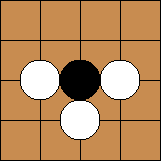
\includegraphics[width=\textwidth]{ex/Ex1-0.png}
\caption{Before Move}
\label{fig:ex1-0}
\end{subfigure} \qquad\qquad
\begin{subfigure}[b]{0.30\textwidth}
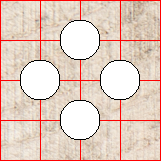
\includegraphics[width=\textwidth]{ex/Ex1-1.png}
\caption{After Move}
\label{fig:ex1-1}
\end{subfigure}
\caption{The black stone is “captured” when the white stone is placed at the top because the black stone loses its last liberty}
\label{fig:ex1}
\end{figure}

The basic rules of Go are as follows:
\begin{enumerate}

  \item Initial Go board is empty containing no stones unless handicaps are applied.
  \item Black plays first and then white. Players take turns alternately placing a stone of their colour.
  \item The board contains a 19x19 gridline pattern with 361 intersections. Stones are played on the intersections and not the square in between. Stones can only be played on empty intersections. These intersections are also referred to as points on the board.


  \begin{figure}[!ht]
  \centering
  \begin{subfigure}[t]{0.20\textwidth}
  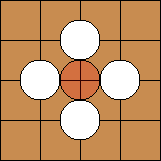
\includegraphics[width=\textwidth]{ex/Ex2-0.png}
  \caption{Middle point is invalid for black to play}
  \label{fig:ex2-0}
  \end{subfigure}  \qquad\qquad
  \begin{subfigure}[t]{0.30\textwidth}
  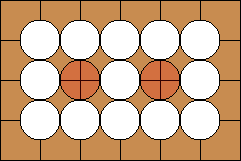
\includegraphics[width=\textwidth]{ex/Ex2-1.png}
  \caption{Both middle points are invalid for black to play}
  \label{fig:ex2-1}
  \end{subfigure}
  \caption{A black stone cannot be placed in the middle of both of these shapes because it would lead to self-capture.}
  \label{fig:ex2}
  \end{figure}

  \item Each turn consists of few parts as follows:
  	\begin{enumerate}[label={(\alph*)}]
		\item Current player is to place a stone of their colour on an empty intersection of their choice.
		\item Then any opponent stones that do not have a liberty are removed from the board. See ~\autoref{fig:ex1}.
		\item A move is invalid if it will cause one or more stones of the current player to be captured – this is to prevent self-capturing moves. See ~\autoref{fig:ex2}.
		\item Removal of the opponent’s stones takes precedence over the self-capture check. This allows for moves which capture opponent’s stones which is otherwise sucidal if the opponent’s stones are not removed first. See ~\autoref{fig:ex3}.
	\end{enumerate}

    \begin{figure}[!ht]
    \centering
    \begin{subfigure}[b]{0.30\textwidth}
    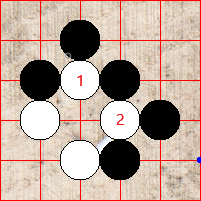
\includegraphics[width=\textwidth]{ex/Ex3-0.png}
    \caption{Before Move}
    \label{fig:ex3-0}
    \end{subfigure} \qquad\qquad
    \begin{subfigure}[b]{0.30\textwidth}
    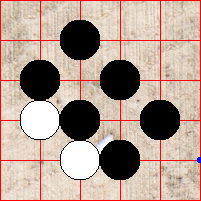
\includegraphics[width=\textwidth]{ex/Ex3-1.png}
    \caption{After Move}
    \label{fig:ex3-1}
    \end{subfigure}
    \caption{A black stone can be placed in the middle of the four white stones because 1 and 2 will be immediately captured before the self-capture rule is applied. }
    \label{fig:ex3}
    \end{figure}

    \begin{figure}[!ht]
    \centering
    \begin{subfigure}[bt]{0.30\textwidth}
    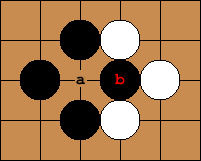
\includegraphics[width=\textwidth]{ex/Ex4-0.png}
    \caption{Before Move}
    \label{fig:ex4-0}
    \end{subfigure} \qquad\qquad
    \begin{subfigure}[bt]{0.30\textwidth}
    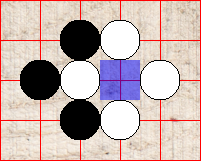
\includegraphics[width=\textwidth]{ex/Ex4-1.png}
    \caption{After - Blue Square is Ko}
    \label{fig:ex4-1}
    \end{subfigure}
    \caption{ Once a white stone is placed at a to capture the black stone at b, a black stone cannot be played at b next turn by the opponent to capture the white stone placed at a.}
    \label{fig:ex4}
    \end{figure}

  \item Ko rule – Player is not allowed to place a stone on point A if it will capture exactly one opponent stone which was placed on point B during the opponent’s previous turn. This rule only applies if the opponent in the previous turn captured exactly one stone on point A. This is to prevent an infinite repetition of the same few moves. See ~\autoref{fig:ex4}.

  \item The game is over when both players pass consecutively and the player with more territory wins. (Scoring can be complicated but is irrelevant to understand the basic rules)

\end{enumerate}




\section{Rules for Go-LD}
The previous section outlines all the essential rules of Go. Some of these rules are slightly altered in order to suit the problem-solving environment set in Go-LD.

The alterations are as follows:
\begin{enumerate}

\item The initial board is set up to represent a Life and Death problem - should be a \bo{valid initial board position}.
\item Not all 361 intersections can be played on – boundaries are set by the creator of the problem.
\item For the purpose of these problems, one player is considered to be the attacker and the other to be the defender.
\item Attacking player is not able to pass unless they have no valid moves and the Ko rule is restricting play.
\item Two consecutive passes do not end the game/problem.
\item The problem is solved when they attacking player has no valid moves and cannot pass, if the keystones are still on the board then the defending players have won. Otherwise, the problem is solved when all the keystones are captured hence the attacking player has won.

\end{enumerate}


\bigskip
A \bo{valid initial board position} is defined by the following :
\begin{itemize}
\item Contains at least one keystone
\item All keystones are the same colour
\item Must have a valid empty intersection to play on within the boundaries set for the problem
\item Can only contain up to one point of Ko
\item Stones that have no liberties cannot exist on the board
\end{itemize}

\bigskip
The reason behind the 4th alteration to the basic rules is to restrict infinite passing which would be allowed due to the 5th alteration. Attacking player is allowed to pass under the circumstance that they have no valid moves and an empty intersection is invalid to play on due to the Ko rule, this resolves some rare occurrences where boundaries set by the creator of the problem restricts the attacking player from winning.

\subsection{Boundaries}
A standard game of Go is played on a 19x19 board where every intersection on the board is playable if the rules of the game allow it. The implications of the size of the board for this project and for computer Go in general is that the search space is too large to obtain good results in a short period of time even with a depth limited search.

There was a definite need for boundaries to be set on the board for each problem to achieve the aim of this project. Without doing so, the number of valid moves required to be searched by the computer would be too large to determine the best move in a limited time. Setting boundaries allow the computer to solve more problems.

The drawback of adding boundaries is that problems themselves become substantially easier compared to the same problem with no boundaries. Boundaries limit the options given to the computer hence increasing the chance of it finding the correct answer. For the computer to solve a difficult problem with no boundaries and therefore have more than 300+ moves to search through is an unachievable task using standard search algorithms. In comparison for the computer to solve the same problem with boundaries which limits the possible moves to less than 20 is a much simpler task which could be done in a reasonable time.

To set boundaries during the creation of a problem, the creator can deem which points are relevant for the problem by placing “valid points” on the board. Any points on the board with preplaced stones are also regarded to be within the boundary. For example, if a black stone is captured then the empty point remaining will be regarded within the boundary of play. Ideally, the creator of the problem should distribute “valid points” in a way to maintain the same level of difficulty for human players but also limit the number of intersections for the computer to search through. It can be very difficult or even impossible for a problem creator to determine all the relevant points for the problem. Go-LD leaves it in the hands of the problem creators to define Life and Death problems with appropriate boundaries. This is a crucial trade-off which is required to allow the program to be able to find the correct answer in a feasible time.



\section{Go-LD Terminology}

Throughout this dissertation many terms are used to describe various aspects of Go, some of which are commonly used terms within the Go world and others were created for the purpose of this project.

Keystones – Set of predetermined stones which are used as markers for groups of stones which are the objective of the problem. These stones are to be captured by the attacking player and kept alive by the defending player.

Attacking player – In terms of Life and Death problems, the attacking player is the player who is trying to capture the keystones on the board.

Defending player – In terms of Life and Death problems, the defending player is the player who is trying to keep the keystones alive on the board.

Board position – Refers to the entire state of the board, not just a single point on the board. Includes Ko points, whose turn it is and all the stones on the board.

Valid points – Set of predetermined intersections that are allowed to be played on for the given problem. A valid point/move can also refer to a point which the current player is able to play on according to the rules.

Connected - Two stones are connected if they are of the same colour and are adjacent to each other or there is a set of stones of the same colour which is connected to both stones.

String – Set of stones of the same colour which are directly connected.

Keystring – Any string which contains one or more keystones.

Group - A broader term used to decribe a collection of stones of the same colour, meaning changes depending on the context.


\begin{figure}[!ht]
\centering
\begin{subfigure}[b]{0.20\textwidth}
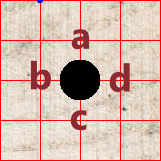
\includegraphics[width=\textwidth]{ex/Ex5-0.png}
\caption{One Stone's liberties}
\label{fig:ex5-0}
\end{subfigure}\qquad\qquad
\begin{subfigure}[b]{0.30\textwidth}
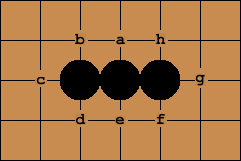
\includegraphics[width=\textwidth]{ex/Ex5-1.png}
\caption{Stone string's liberties}
\label{fig:ex5-1}
\end{subfigure}
\caption{The liberties of a stone or a string of stones are the empty adjacent intersections.  In ~\autoref{fig:ex5-0} intersections \bo{a},\bo{b},\bo{c} and \bo{d} are the liberties of the black stone.
In ~\autoref{fig:ex5-1} intersections \bo{a} to \bo{g} are the liberties of the black stone string but \bo{h} is not a liberty due to the white stone that occupies it.}
\label{fig:ex5}
\end{figure}



Liberty - The liberties of a stone are all the adjacent empty intersection of the stone and all adjacent empty intersection of any stone connected to the original stone. See ~\autoref{fig:ex5}.





Atari – String is in Atari when it only has one liberty.

Atari Point – The last remaining liberty of a string.

Ko Point –  An empty intersection which is restricted from play due to the Ko rule

Seki – Two strings of opposing colours that are alive next to each other. Neither player can capture the opponent string without first sacrificing their own string.





\section{Life and Death Problems}

Life and Death is an essential part of Go. Life and Death is the term used to describe the battle that takes place to either attack and capture enemy stones or to defend and keep alive one's stones.  These situations on the board where it becomes crucial to defend one’s stone strings or capture enemy ones arrive very often. During the end game in Go, the ability to win these battles with as much territory as possible will decide the victor. Beginners are highly recommended to understand and learn how to play out these battles as they are clear deciders of the game. Much of the literature on Go is purely based around providing Life and Death problems and explaining the importance of them and how to tackle such situations appropriately \citep{Cho1993}\citep{Davies1975}. The purpose of Go-LD is to create a tool which helps players to understand and solve these problems.

\subsection{Dead, Alive or Unsettled}

The three main ways to describe the status of a string are alive, dead or unsettled. To deduct the state of a group of stones accurately can be difficult. Doing so requires a lot of experience and knowledge about the possible moves that could be made and the counter plays to them.

\begin{figure}[!ht]
\centering
\begin{subfigure}[b]{0.45\textwidth}
\includegraphics[width=\textwidth]{LD/1a.png}
\caption{Before Moves}
\label{fig:LD-1a}
\end{subfigure}\qquad
\begin{subfigure}[b]{0.45\textwidth}
\includegraphics[width=\textwidth]{LD/1b.png}
\caption{After Moves}
\label{fig:LD-1b}
\end{subfigure}
\caption{Straight Four in the corner is alive}
\label{fig:LD-1}
\end{figure}

A group of stones are said to be alive if the group cannot be captured even if the opponent is to play first. To expand on this, even if the opponent plays a move which threatens the group of stones there is always a responding move which will, in turn, keep the group of stones alive. ~\autoref{fig:LD-1} shows an example of a white group which can be deemed to be alive. If black first plays at \bo{1} then white will play at \bo{2}, if black first plays at \bo{2} then white will play at \bo{1}; both outcomes will lead white group having two eyes and therefore alive. Eyes are explained in the next section.

\begin{figure}[!ht]
\centering
\begin{subfigure}[b]{0.3\textwidth}
\includegraphics[width=\textwidth]{LD/2a.png}
\caption{Before Moves}
\label{fig:LD-2a}
\end{subfigure}\qquad
\begin{subfigure}[b]{0.3\textwidth}
\includegraphics[width=\textwidth]{LD/2b.png}
\caption{After Moves}
\label{fig:LD-2b}
\end{subfigure}
\caption{Square Four in the corner is dead}
\label{fig:LD-2}
\end{figure}


A group of stones is said to be dead if the group can be captured even if the group’s colour can play first. For example, a white group is deemed dead if white can play the first move and black has a responding move which will keep the white group in a dead state. ~\autoref{fig:LD-2} shows a group of dead white stones, for this group to live, it would require two white stones on two points diagonally opposite to each other and no white stones on the other two points. For example, if white can play at \bo{a} and \bo{d} then it becomes alive. This is impossible to achieve as black can respond to white’s initial move by playing at the diagonally opposite point as seen in~\autoref{fig:LD-2b}.


A group of stones is said to be unsettled when the group is alive if the group’s colour can play first but dead if the opponent plays first. Groups which are unsettled are crucial to the outcome of the board, whoever can play first near the group can determine who controls the whole territory the unsettled group surrounds. ~\autoref{fig:LD-3a} shows an unsettled white group which has a vital point at \bo{a}. If white plays first at \bo{a} then the group achieves two eyes and is alive. On the other hand, if black plays at \bo{a} first then white cannot achieve two eyes, hence it becomes dead.

\begin{figure}[!ht]
\centering
\begin{subfigure}[b]{0.4\textwidth}
\includegraphics[width=\textwidth]{LD/3a.png}
\caption{Vital point at a}
\label{fig:LD-3a}
\end{subfigure}\qquad
\begin{subfigure}[b]{0.4\textwidth}
\includegraphics[width=\textwidth]{LD/3b.png}
\caption{White lives with 2 eyes}
\label{fig:LD-3b}
\end{subfigure}
\caption{Straight Three on the side is unsettled}
\label{fig:LD-3}
\end{figure}




\subsection{Eyes}
The concept of an eye is critical in understanding Life and Death problems and Go in general. There are no correctly defined statements on what an eye is but in general, an eye is an empty space surround by a group of the same colour. Single eye point shapes are shown in ~\autoref{fig:LD-4}. In these shapes, the stones surrounding the eyes are essential if any of them are missing then the eye will no longer be a real eye hence the shape is much weaker. The opponent cannot play on a single point eye unless the eye is the only liberty of the surrounding stones. If a group of stones contains two real eyes, then it becomes impossible to capture that group of stones unless the eyes are covered up by its own colour of stones. These groups of stones are unconditionally alive which means even if the opponent can play multiple times in a row the group cannot be captured. ~\autoref{fig:LD-3b} shows an example of a group of white stone which contains two eyes at \bo{a} and \bo{b}. Due to the self-capture rule black can never place a stone at \bo{a} without having a stone at \bo{b} and the same applies for \bo{b} hence the white group in unconditionally alive.

\begin{figure}[!ht]
\centering
\begin{subfigure}[b]{0.3\textwidth}
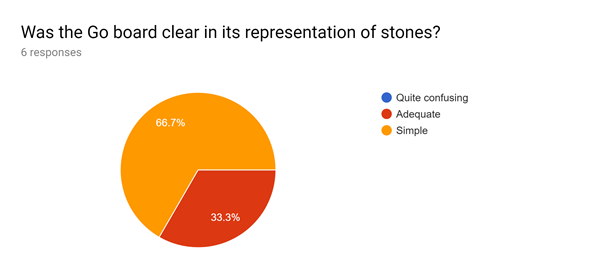
\includegraphics[width=\textwidth]{LD/4.png}
\caption{Different Single Point Eyes}
\label{fig:LD-4a}
\end{subfigure}
\caption{Single Point Eye in the middle, side and corner}
\label{fig:LD-4}
\end{figure}



In cases of larger groups which surround more empty points, these empty points are referred to as the eye space. The eye space of a group is vital in determining early on within a game whether a group is dead or alive. An eye space can be reduced to create real eyes; the larger the eye space a group surrounds the greater the ability it has to create two real eyes and live unconditionally.

When eyes are not fully developed on the board for instance at \bo{a} in ~\autoref{fig:LD-5a} they are deemed to be half eyes. Depending on who plays first at \bo{b} decides whether a real eye is formed or is stopped from being formed. Half eyes are important because two half eyes add up to one real eye.  The group presented in ~\autoref{fig:LD-5b} has a real eye at \bo{a} and two half eyes at \bo{b} and \bo{c}. This group can be deemed as alive because when black plays \bo{1} to deform a half eye white can play \bo{2} to fully form the other half eye into a real eye creating an unconditionally alive group.

\begin{figure}[!ht]
\centering
\begin{subfigure}[b]{0.4\textwidth}
\includegraphics[width=\textwidth]{LD/5a.png}
\caption{Vital point at a}
\label{fig:LD-5a}
\end{subfigure}\qquad
\begin{subfigure}[b]{0.5\textwidth}
\includegraphics[width=\textwidth]{LD/5b.png}
\caption{White lives with 2 eyes}
\label{fig:LD-5b}
\end{subfigure}
\caption{Straight Three on the side is unsettled}
\label{fig:LD-5}
\end{figure}


\subsection{Outcomes of Life and Death}
The possible outcomes of some Life and Death situations are not as obvious it would seem. There are different types of Life and Death results. The varying types of result for a problem can vary the outcome of the whole board.

Unconditional life or escape into the centre of the board is the best outcome a defending player can expect; this means their group of stone will be scoring them points without uncertainty.

Another but a lesser type of victory for the defending player is life through Seki, which means mutual life, this is where two groups of opposing colours of stones live sharing liberties. Neither player can try to capture the opponent’s group because it will lead to their group’s death first. When an attacking group of stones can live in mutual life along with the defending player’s group then the outcome is slightly less favoured than unconditional life due to the end game scoring. In isolated Life and Death problems and for Go-LD this difference between unconditional life and Seki is not taken into account, Seki is deemed to be victory for the defending team.

Life and Death problems can also conclude where Ko occurs within the area. In a full game of Go this is very important in deciding Ko fights in other parts of the board and can be seen as leverage to be used.  For Go-LD and in isolated problems these situations are played further on until a defining end is met where the group is dead or alive.

The final possible result is death where the defending player’s group is captured without any Ko situation occurring which the best-case scenario for the attacking player.

\section{Related Works}

Martin Müller's Explorer \citep{Muller2002} was a strong program developed with the intention of playing Go. In his paper, he delves into some key aspects of Explorer which have been useful to comprehend some ideas behind creating a Go-playing software. He describes the importance of board evaluation within a tree search algorithm such as Minimax.

Explorer can evaluate certain areas of the board in terms of safe territories for each player and can distinguish between safe stones and safe territories. Safe stones are any stones that are deemed alive but safe territories requires that opponent stones cannot live within the safe stones' territory. Explorer also takes into consideration of Semeai positions which are capturing races that occur within Go. The victor of Semeai can be determined early sometimes and hence doing so during the evaluation could save searching further during a tree search algorithm. Müller also goes into detail about his zone-based evaluation where Explorer can distinguish areas which are in conflict and areas which are clearly controlled by a certain player.

While Explorer aims to play Go, this project aims to create a program to solve Life and Death problems. To do so, determining the safety of keystrings within a problem can be helpful. Explorer's methods of recognising safe strings such as Benson's algorithm \citep{Benson1976} and also the improved version of the algorithm described in Müller's previous work \citep{Muller1998} were regarded during the initial design of Go-LD.

Work done by Ken Chen and Zhinxing Chen \citep{Chen1999} in creating Go Intellect and HandTalk were also quite interesting and relevant while working on this project. Their work regarding eyes and determining the value of a shape of stones depending on the number of eyes the shape can produce was great a motivator during the implementation of Go-LD's pattern-based heuristics.

Another relevant work researched during this project was Adrian B. Danieli's paper on his own TsumeGo problem solver \citep{Adrian2010}. In his paper, he explores in-depth the process in which his program was developed. Explanation of key concepts such as move generation and board evaluation helped to understand how to develop Go-LD. A particularly relevant piece of information which was used as advice during the design of Go-LD was that there was a problem in his representation of each node during the tree search. He believed his representation of each node caused extra workload during tree search without a good reason to do so. He goes on to explain due to the depth-first nature of his program "compressing" and "decompressing" the board positions for every node was a waste of time. Rather than saving some space which is not as relevant when using a depth-first search, it would have been better to save time by storing the entire board position for each node.








\chapter{Requirements \& Software Development}

The project needed a well-defined list of requirements to outline key features and help determine the implementation order of those key features. Time constraints and the resources available had to be taken into consideration before further work on the project was done. The functional requirements identified earlier on the project captured most of the work required. Throughout the project, these requirements were refined and expanded upon to solve unseen problems that arose during the project. Also, some non-functional requirements were also discovered earlier on which were used to refine the goals of the project even further.

\section{Functional Requirements}

The program was split into to three core parts from the beginning of the project : play mode, editor mode and the “computer”. Hence splitting the functional requirements into the following sections was ideal.

\subsection{General Requirements Across Both Modes}
There were many requirements which were common between play mode and editor mode, to reduce redundancy it is better to express them together.

\subsubsection{Go Board}
The Go board is an integral part of both modes and is required for the user and the computer to interact with the program. A board object which is capable of storing relevant data and contained methods which can process the relevant data was essential.

The relevant data required includes the following:
\begin{itemize}
\item A representation of all the points on the board
\item Current turn
\item All of the stone strings for both colours
\item Colour of keystone
\item Point of Ko
\item Lists of Atari points for both colours
\item List of valid moves for the current turn
\end{itemize}

The relevant methods which are able to do the following were also required:
\begin{itemize}
\item Make a move on the board and update the entire board accordingly
\item Generate all the valid moves for the current player
\item Check if a move is valid – this should include self-capture check and Ko check
\item Check for capture and remove stones accordingly
\item Obtain all the liberties of a given stone string
\end{itemize}

\subsubsection{Other Features}
Along with the Go board, play mode and editor modes had multiple features which were required to allow the users to perform simple tasks.

Both modes needed the following features implemented:
\begin{itemize}
\item Load problem
\item Save problem
\item Switch modes
\item Undo \& Redo moves
\end{itemize}

\subsection{Play Mode}
The play mode required some unique features which allowed the user to play through problems and also to adjust the computer’s settings.

Play mode needed the following features most likely in the form of a button:
\begin{itemize}
\item Request the computer to start search for the best move
\item Request the computer to stop search
\item Pass
\item Swap turns
\item Reset the problem to when it was loaded
\item Set whether the computer responds automatically to user’s move or not
\item Set the breadth limit for the search
\item Set the depth limit for the search
\end{itemize}

\subsection{Editor Mode}
The editor mode required some unique features to allow the users to create and edit  Go problems with ease.

Editor mode needed the following features most likely in the form of a button:
\begin{itemize}
\item Set who plays first during the problem
\item Reset the board into an empty state
\item Rotate and flip the board
\item Place keystone
\item Switch keystone colour
\item Choose which colour of stone to place
\item Remove stones
\item Set and remove “valid points”
\end{itemize}

\subsection{The Computer}
The main aim of the project required the computer to perform a tree search. The tree search chosen for this project was the Alpha-Beta pruning algorithm. The requirement for the computer was that it needed to be able to find the best move possible and play it on the board in a limited time frame. This needs to be done through a tree search where many valid sequences of moves are searched through, and the move which results in the best board position for the current colour needs to be played. An additional requirement for the computer was that it should be able to limit the depth of the search according to the user’s choice. This consequently implies a requirement for a board evaluation function which is used to score the board positions found at the depth limit. The computer was also required to have the ability to limit the breadth, i.e. the number of moves per ply to be searched, according to the user’s choice. Hence there was a need for a move generator to produce a subset of moves from all the valid moves.


\section{Non-Functional Requirements}
Throughout the project, some non-functional requirements were discovered and needed to be addressed. The following categories were used to specify the different criteria Go-LD need to achieve.

Performance / Time - A significant concern was the time a user wants to spend during the process of solving problems. For example, the time it took for the computer to make a move had to be reasonable.

Usability - Another concern was the ease of use, whether the program is simple and understandable for untrained users.

Reliability – The program should be able to cope with any user inputs and should maintain running without any failures or crashes.

In order to test all three categories of these non-functional requirements the project also had an additional requirement of producing a folder of problems which can be used during the evaluation phase. This folder of problems was required so that beta testers could have a set of pre-defined problems to test the program on. The folder was also required to perform quantitative evaluation of Go-LD during the evaluation process, to judge the level of difficulty the computer can solve and what length of time it takes to do so.

\section{Software Development Process}
From the start, the project was divided into two major milestones each containing a set of requirements to achieve the milestone. These milestones were set up to help evaluate the progress throughout the project and also to help streamline the workflow throughout the project so that at all points there was a goal to strive towards.

\subsubsection{Milestone 1}
The first milestone consisted of creating and implementing most of the essential features of the program. The first choice made during the project was to choose Java as the primary programming language within the project. This choice came entirely out of preference and ease of use. Once this was determined a 2D graphics engine was required to draw the program. Initially, to immediately start work on the project, the Swing tool kit along with Java’s Canvas was used. After further development and research, it was found that this combination of tools kits was insufficient for the project. From there onwards the  \cite{SLICK2D} ,a graphics tool kit, was used to render the program.

The first milestone came with the challenge of implementing a tree search. The final tree search used within Go-LD was created after two iterations of designing and implementing a tree search. The first iteration was based on the Minimax tree search algorithm which was adapted to play Go. The next iteration of the tree search consisted of Alpha-Beta pruning tree search which greatly improved the performance compared to the simple Minimax search. Finally, to improve the quality of the overall program in terms of usability and to improve performance, Iterative Deepening was used along with Alpha-Beta. Note that Iterative Deepening was implemented much later on the project and was part of the second milestone.

\subsubsection{Milestone 2}
The second milestone was concerned with implementing heuristics within Go-LD. Which  included board evaluation, move generation and move ordering. Board evaluation features were the first of the three to be designed and implemented because it was arguably the most important of the three and required the most time and effort.

To implement board evaluation research was done about Go and how humans perceive the value of different Go board positions. Countless hours were spent understanding some of the essential strategies regarding eyes and alive shapes and dead shapes. A lot of the information gathering was done through Sensei’s Library, a website \citep{Senseis} which has information on almost every aspect of Go from simple to advanced. The result of research inspired the pattern matching based board evaluation used within Go-LD.

Once the board evaluation function became sufficient enough to solve moderately difficult problems, the focus was set on move ordering. At this point, the Killer Move heuristic was already thoroughly explored when the research was done about Alpha-Beta. Hence it was a simple matter to apply it to Go and implementing it within the search. When Iterative Deepening was introduced, it was merely a matter of some alteration to the code to implement move ordering using the Principal Variation of each previous iteration. This was also essential to keep the performance of Iterative Deepening comparable and sometimes better than a fixed-depth search.

The final part of the program to be implemented was the move generator. It was essential that this was kept simple as it is used during every ply of the search. Hence a complex move generator would drastically slow down the performance. To keep it simple a distance-based generator was designed, which prioritised moves nearer to keystones. After implementation and testing the distance-based generator was found to be inadequate to generate moves for more spread-out Go problems. Therefore, a pattern-matching based move generator was designed and implemented combined with the distance-based generator to yield better results.








\chapter{Design}


\section{Tree Search}
Go-LD allows the user to play against the computer which is one of the main requirements of the project.  Go-LD must be able to determine the best move out of all the valid moves for the current board position to create a computer which can play against a human and solve problems. The simplest way to achieve this is by searching through the game tree and determining the result of each valid sequence of moves. The game tree consists of every single board position that can occur from the current board position. The board position refers to the state of the board, where each stone is on the board, whose turn it is and also if there is an intersection of the board where the Ko rule is applied. Each subtree of the game tree is the result of making a valid move in the current board position. Every subtree of the current board position needs to be explored until a game-ending state to determine the best move.

\subsection{Minimax}
The method of finding the correct move within Go-LD is the Alpha-Beta pruning search algorithm which is based on the Minimax search algorithm. A simple implementation of Minimax with no depth limit will search each valid move of the initial board position until a gaming-ending state occurs. Minimax will choose a move which results in victory even if the opponent plays optimally if such a move exists.

\begin{figure}[!ht]
\centering
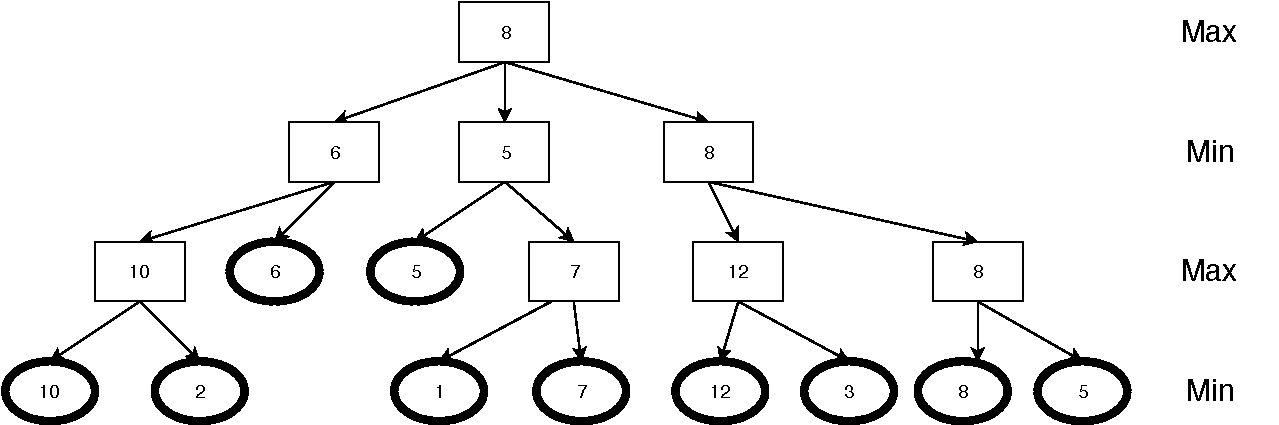
\includegraphics[width=0.9\textwidth]{MinMaxNumTree.pdf}
\caption{Minimax used for simple number game. Best score the maximizing player can get is 8. Even though scoring 10 and 12 are possible if the minimizing player plays optimally these scores cannot out be achieved.}
\label{fig:MinMaxNumTree}
\end{figure}

\subsubsection{Game-Ending State}
Go-LD is only concerned with Life and Death situations in Go hence it is simple to determine if the current board position is a game-ending state. If the attacking player has no valid moves and the keystones, marked by the problem creator, remain on the board then the defending player has won. Alternatively, as soon as the attacking player captures all the keystones, they win. In a real game of Go, the result of Life and Death situations is not as simple. There might be multiple solutions which result in the capture of all the keystones, but there might only be one solution which will do so without allowing losses on other parts of the board for the attacking player. These kinds of difference in result are ignored within Go-LD as we are only interested in the result of the Life and Death problem, and not the outcome of the board. Hence any solution which captures all the keystones are sufficient for the program.

~\autoref{fig:MinMaxNumTree} shows an example of Minimax for a simple game where the max player tries to obtain the highest value and the min player tries to obtain the lowest value. Note an oval shape represents a game-ending state.

\subsection{Alpha-Beta Pruning Search}
The Alpha-Beta pruning algorithm is a smart improvement on the Minimax algorithm in order to reduce the search time. It determines the same result without having to search through as many subtrees as Minimax does. It uses alpha and beta values to determine whether searching a subtree further is a waste of effort or not. The search begins with the alpha value set to -inf and the beta value set to +inf. These values are passed down from the parent tree to each of its subtrees during the search. If a maximising subtree finds a move which results in a score higher than the previous best score for that board position, then the alpha value of that subtree is increased to the value of the new best score. If a minimising subtree finds a move which results in a score lower than the previous best score for that board position, then the beta value of that subtree is decreased to the value of the new best score. After searching each move within a subtree, the algorithm checks if the alpha value is greater than or equal to the beta value and if it is then the algorithm decides that searching more moves within that subtree is pointless and returns the best score found so far back to the parent tree. These “alpha-beta cut-offs” reduces the search space for the algorithm by cutting off the rest of the moves of that subtree from being searched. Reduction in search space amounts to a significant improvement in search time compared to the Minimax algorithm without changing the result. The results do not differ because the move that caused the alpha-beta cutoff to occur is worse than the parent tree’s best move found so far.

\begin{figure}[!ht]
\centering
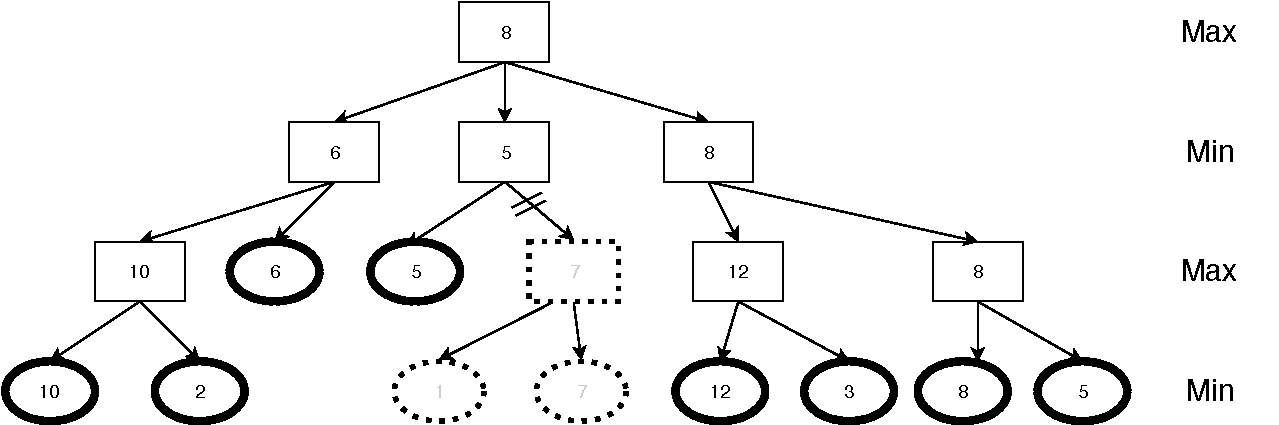
\includegraphics[width=0.9\textwidth]{ABNumTree.pdf}

\caption{The same simple number game as ~\autoref{fig:MinMaxNumTree} but using Alpha-Beta pruning. In the second subtree after searching the first move which returns 5, the algorithm cuts off from any further search in that subtree as it realises the first subtree will always be better than 5. }
\label{fig:ABNumTree}
\end{figure}


\subsubsection{Limiting Depth}
A non-depth limited Alpha-Beta search will search deeper and deeper until a game-ending state is found; this is very impractical for larger problems. Note that “depth” and “deeper” refers to how many moves ahead the computer searches, the higher the depth the further ahead the computer has searched. Best way to deal with this is to introduce a depth limit where once depth x is reached the search is not continued. The problem with this is that when these depth cut-offs occur the board position will not be in a game-ending state. Therefore, the Alpha-Beta search needs to do some type of board evaluation to determine the value of the current board position, board evaluation used within Go-LD is detailed further on the chapter.

\subsubsection{Go Adapted Alpha-Beta Pseudocode}
The following pseudocode addresses the Alpha-Beta pruning search algorithm with Go's Life and Death problems in mind. It was used for the initial design of Go-LD's move finder function and later adapted to implement heuristics described in the following sections of this chapter.

\begin{algorithm}[H]
\caption{Alpha Beta Pruning Search}\label{Alpha-Beta}
    \DontPrintSemicolon
    \SetKwFunction{FalphaBeta}{alphaBeta}
    \SetKwProg{Pn}{Procedure}{:}{}
    \Pn{\FalphaBeta{$board,isDefending,depth,alpha,beta$}}{
         $depth\gets (depth+1)$\;
         $validMoves\gets (board.validMoves)$\;
        \uIf{keyStones.size = 0}{$\KwRet -\infty\;$}
        \uIf{(board.turn = attacking \textbf{and} validMoves.size = 0)}{$\KwRet { }\infty\;$}

        \eIf {isDefending}{
            $best\gets -\infty$\;
            \ForEach{move in validMoves}{
                board.makeMove(move)\;
                $score \gets alphaBeta(board,!isDefending,depth,alpha,beta)$\;
                board.undoMove()\;
                \lIf {($depth = 1$  \textbf{and}  $\mbox{score}<\mbox{best}$)}{$bestMove \gets move$}
                $best \gets max(best,score)$\;
                $alpha \gets max(alpha,score)$\;
                \lIf {$beta \leq alpha$}{$break$}
            }
            {$\KwRet { }best\;$}
        }{
            $best\gets \infty$\;
            \ForEach{move in validMoves}{
                board.makeMove(move)\;
                $score \gets alphaBeta(board,!isDefending,depth,alpha,beta)$\;
                board.undoMove()\;
                \lIf {($depth = 1$  \textbf{and}  $\mbox{score}>\mbox{best}$)}{$bestMove \gets move$}
                $best \gets min(best,score)$\;
                $alpha \gets min(alpha,score)$\;
                \lIf {$beta \leq alpha$}{$break$}
            }
            {$\KwRet { }best\;$}
        }
    }
\end{algorithm}


\subsection{Alpha-Beta with Iterative Deepening}

Due to the depth-first nature of a fixed-depth limited Alpha-Beta search, the search will not provide a result until every move is searched to a game-ending state or the limited depth. This means the search will not be able to produce the best move searched so for if it is stopped in the middle. Without the introduction of Iterative Deepening in Go-LD’s search the user is not able to search for a limited amount of time, instead, the user would have to predict which depth limit to set in order for the search to complete in the time they desire. Predicting the depth limit could lead the user to set the depth limit too high which would lead the search to last longer than what the user would prefer. Iterative deepening fixes this issue by allowing the user to stop the search whenever they desire and to use the result of the last completed iteration to make the best move found so far hence improving the usability of the Go-LD.

Alpha-Beta with Iterative Deepening is a process in which the search is performed multiple times, and at each iteration, the depth limit is increased by 1. This cycle takes place until max depth limit is reached, or a favourable game-ending state is found. Iterative Deepening effectively alters Alpha-Beta search to only increment depth by one at a time.  ~\autoref{fig:iter-deep} illustrates the process of Iterative Deepening, it is essential to understand that Iterative Deepening is not a new search algorithm itself but rather a framework which contains the Alpha-Beta search.


\begin{figure}[!ht]
\centering
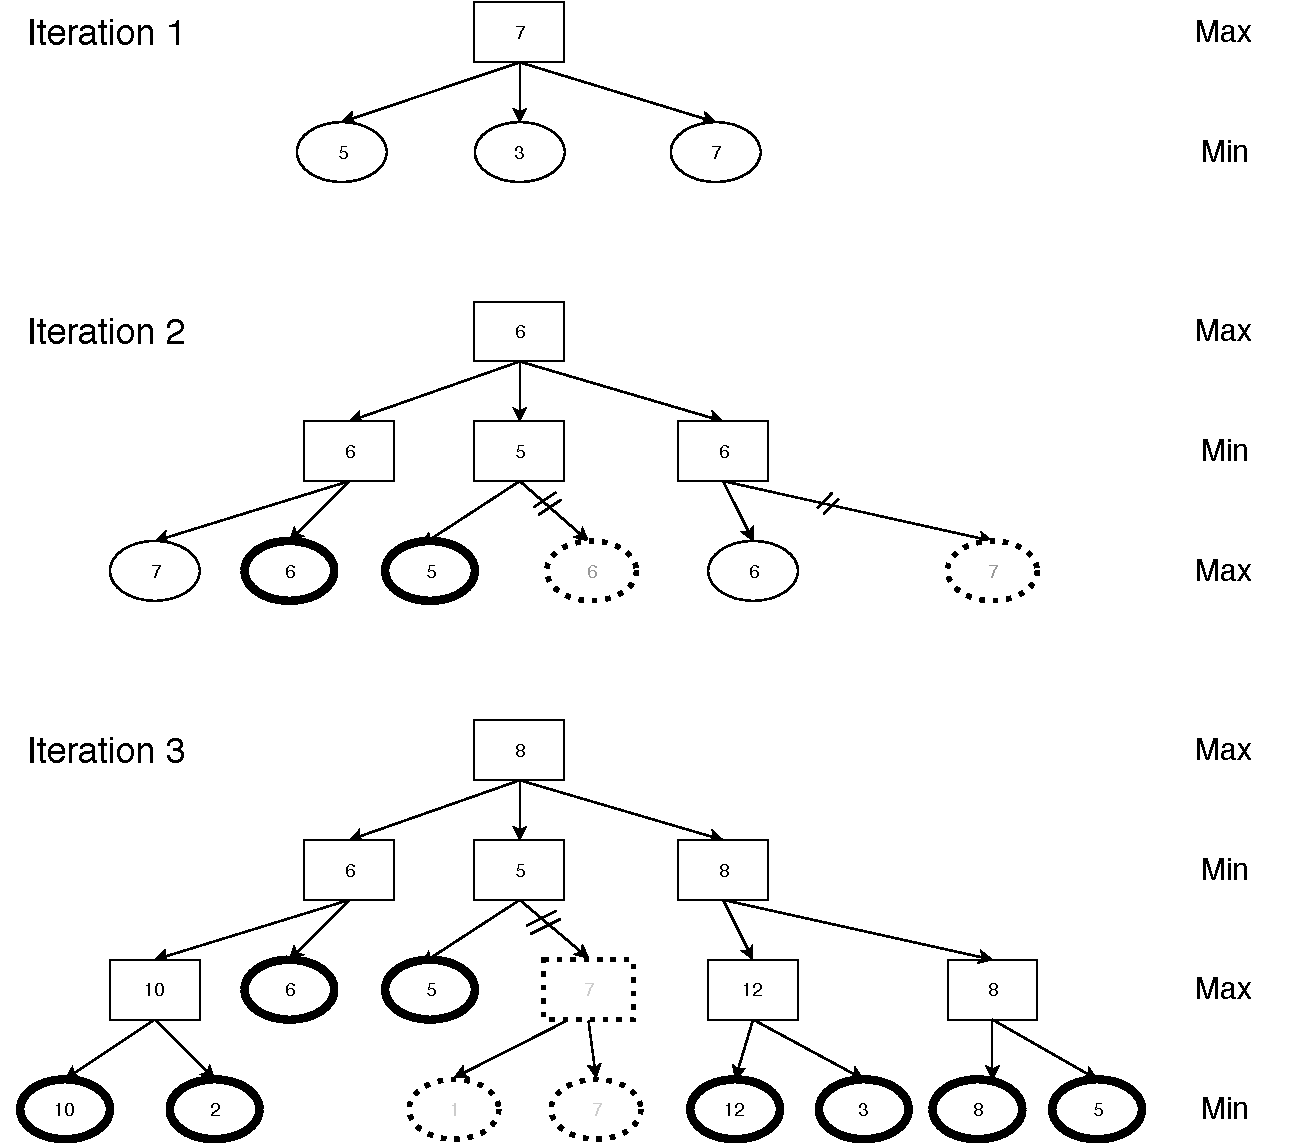
\includegraphics[width=0.9\textwidth]{ABNumIDeep.pdf}
\caption{ The same simple number game as ~\autoref{fig:ABNumTree} but using Iterative Deepening. Note here the thinner oval shapes represents an evaluated state due to depth limitation. Whereas the emboldened oval shapes represent a game-ending state. End of each iteration there is a resulting answer which the search can return if the user decides to stop in the middle of the search.}
\label{fig:iter-deep}
\end{figure}


The drawback of this process is that it requires multiple iterations of the Alpha-Beta search and which will be required to perform redundant computation for the lower depths of the game tree. Work done by Richard E.Korf  shows that redundant computation does not affect the overall time of the tree search as much as it would seem. Using the result of each iteration to perform the next iteration can reduce the time taken to perform the next iteration and the overall run time of the search \citep{Korf1985}. The Principal Variation move ordering heuristic is based on this idea, explained later on in this chapter.




\section{Heuristics}

The Alpha-Beta pruning search algorithm by itself is a significant improvement over the standard Minimax algorithm, but even with this improvement, the sheer size of the search space for a game tree can become quickly overwhelming for the search to handle in a reasonable time. Alpha-Beta even at best case has a complexity of $O(\sqrt{b^d})$ and at worst, $O(b^d)$  which means for problems with a higher number of initial valid moves or problems that require to search further ahead to come to a game-ending state could take an endless amount of time to search. For this reason, we have to introduce heuristics to allow the search to come to a quicker solution which might not always guarantee the best move rather than taking a much longer time to find the guaranteed best move. There are quite a few methods of implementing heuristics within the Alpha-Beta search. Go-LD will be able to use a few of these in combination or by themselves to restrict the time taken for the computer to respond to the user.

\subsection{Board Evaluation}
The Alpha-Beta search will have to evaluate the board position when the cut-off depth is reached and return a value which represents how good the board is for the players. For example, if the board position will lead the attacking player to capture all the keystones then the board evaluation should return -5000,   on the other hand, if the board position is in favour of the defending team, then it should return 5000. Creating a function which evaluates the board accurately is a difficult task and doing so which can perform at the level of humans is even more difficult. An essential factor to consider when designing an evaluation function is the time it takes to evaluate a board position. More complex the evaluation function becomes the longer it takes to evaluate single a board position hence the more time it takes to evaluate the board position every time the depth limit is reached.

\subsubsection{Pattern Matching Evaluation}

When evaluating a board position Go-LD looks at the board similar to how humans would look at a board. It tries to identify general patterns on the board to give values depending on the pattern it finds. These patterns are based on the idea of eyes and eyes space. Identifying patterns which will lead to multiple eyes will be evaluated to give a very high score and hence the search will be able to recognise a group of stones which will be able to live without further searching. The general principle behind the patterns used in Go-LD is to identify the number of eyes the pattern can yield when fully played out and values the pattern according to this factor. The value for each pattern found is added to the overall board score.

\begin{figure}[!ht]
\centering
\begin{subfigure}[b]{0.35\textwidth}
\centering
\includegraphics[width=\textwidth]{heur/1a.png}
\caption{Before}
\label{fig:heur-1a}
\end{subfigure}\qquad
\begin{subfigure}[b]{0.35\textwidth}
\centering
\includegraphics[width=\textwidth]{heur/1b.png}
\caption{After}
\label{fig:heur-1b}
\end{subfigure}
\caption{Straight Three in the middle of the board with missing corners.}
\label{fig:heur-1}
\end{figure}


Most of the patterns used within Go-LD have a distinct feature common in Life and Death problems which is that depending on who plays first the pattern/shape becomes dead or alive. In other words, these shapes are unsettled and hence contains vital points which will determine the number of eyes that can be produced by the shape. ~\autoref{fig:heur-1a} shows a pattern used in Go-LD, the shape referred to as Straight Three but with its corner stones missing. The vital point of this pattern is \bo{a} if white can play at \bo{a} then the pattern is almost ensured to create two eyes unless white makes a mistake filling in the corners. The corners \bo{b}, \bo{c}, \bo{d} and \bo{e} are also crucial for this pattern, if black can have stones in both \bo{b} and \bo{c}  or  in \bo{d} and \bo{e} then the wall of shape becomes weak and hence the shape can become captured. Due to alternating play if white plays first in this situation then it will be played out as shown in ~\autoref{fig:heur-1b} where white can produce two real eyes.



\begin{figure}[!ht]
\centering
\begin{subfigure}[b]{0.35\textwidth}
\centering
\includegraphics[width=\textwidth]{heur/2a.png}
\caption{Before}
\label{fig:heur-2a}
\end{subfigure}\qquad
\begin{subfigure}[b]{0.35\textwidth}
\centering
\includegraphics[width=\textwidth]{heur/2b.png}
\caption{After}
\label{fig:heur-2b}
\end{subfigure}
\caption{Bent Three in the corner with a Single Point eye nearby to connect.}
\label{fig:heur-2}
\end{figure}


An essential insight into creating a better evaluation function is to recognise that patterns like the one mentioned earlier will be able to create a single point eye at the worst-case scenario. If the opponent can play at a pattern's vital point and restrict it from creating two eyes, the pattern will still be able to create one real eye which should be also valued quite highly. By connecting two groups each containing one real eye, the defending player can achieve an alive shape. When searched patterns fail to meet two eyes, Go-LD stores the eye space of each failed pattern in a collection of eye spaces. These eye spaces are highly probable to contain one real eye. Once the whole board is searched for all the different patterns used within Go-LD and each identified pattern's values totalled, the evaluating function is left with the collection of eye spaces which all contain one real eye. Using the collection of eye spaces Go-LD is able to group multiple eye spaces which are connected through stones of the same colour. Any group of eye spaces that contains two or more unique eye spaces are identified as highly valuable because they will most likely produce two real eyes.
~\autoref{fig:heur-2} shows an example of where Go-LD can recognise a new shape with two real eyes. Bent Three in the corner is about to lose its vital point once black plays at \bo{a}, but white can connect to the Single Point Eye nearby by playing at \bo{b}. Doing so will create a new shape which contains two real eyes. Go-LD recognises that the Bent Three in the corner will create one real eye even though it has lost its vital point. When white connects at \bo{b}, Go-LD's eye space grouping algorithm identifies that the new shape contains at least two real eyes and hence will score the shape highly.

\begin{figure}[!ht]
\centering
\begin{subfigure}[b]{0.2625\textwidth}
\centering
\includegraphics[width=\textwidth]{heur/3a.png}
\caption{Black Hanes at 1}
\label{fig:heur-3a}
\end{subfigure}\qquad
\begin{subfigure}[b]{0.35\textwidth}
\centering
\includegraphics[width=\textwidth]{heur/3b.png}
\caption{Black Cuts at 1}
\label{fig:heur-3b}
\end{subfigure}
\caption{Important type of moves}
\label{fig:heur-3}
\end{figure}



To limit time spent on board evaluation only a small number of unique patterns can be searched. Due to this constraint, it was essential to identify the fundamental shapes/patterns which can create eyes. Fifteen different patterns ranging from a Single Point Eye to a Rabbity Six along with all their variations on the sides and corners of the board are used within Go-LD.  Along with these patterns, the evaluating function also tries to identify stones which are placed in good positions with respect to the opponent stones. The evaluating function looks for areas of the board that are the result of a cut, hane or even simply connecting two groups of stones and awards values accordingly.


~\autoref{fig:heur-3a} shows a hane which is a move where a stone is placed next to an opponent stone which is already in contact with one’s own stone. Hane is a move which plays around one or more opponent stones. Note: playing at the opposite side of white here is not a hane.~\autoref{fig:heur-3b} shows a cut where black can stop white from connecting the two white stones by playing \bo{1}.





\subsection{Move Ordering}
The benefit of Alpha-Beta pruning search over simple Minimax search is that when alpha-beta cut-offs occur a significant number of subtrees of possible board positions do not need to be searched. Erik van der Werf talks about the importance of move ordering during Alpha-Beta search and the effects of good move ordering heuristics \citep{ErikvanderWerf2004}. If the best move is always selected to be searched first, then the algorithm will produce cut-offs when all the other moves are searched afterwards. The idea behind this is if the best move is found first then all other moves will never return a score which is better than the best move. With this in mind, we can see that ordering the list of moves to consider the best move first or even a move which will produce more cut-offs first, is a great way to reduce the number of board positions to search without altering the result.

\subsubsection{Killer Move Heuristic}
Go-LD uses a deeply researched \citep{Akl1977} method, Killer Heuristic, introduced by Huberman, B.J. to order moves when searching through endgames of Chess using Alpha-Beta. Huberman’s theory \citep{Huberman1968} was that a move (killer move) which led to a better board position from an initial board position \bo{A} will also lead to a better position from a similar initial board position \bo{B} if the move is a valid move for \bo{B}. Using this theory, these killer moves should be searched first when a similar board position occurs during Alpha-Beta search. The moves which are considered killer moves are defined easily by using the cut-off characteristics of the Alpha-Beta search, during the search if a move causes an alpha-beta cut-off to occur then this move can be considered a killer move and hence will be stored to be used for move ordering.  We can define what a similar board position is by merely looking at the depth in which the board position occurs in. Hence an ideal way to implement the killer heuristic is to store some moves for each depth which caused alpha-beta cut-offs to occur. Storing a high number of moves for each depth can lead to increased work during the move ordering process hence it is most effective only to store a few moves. Go-LD only stores two killer moves \bo{k1} and \bo{k2}  for each depth.

Move Ordering for a board position \bo{A} which occurs at depth \bo{d} consists of searching the list of valid moves for \bo{k2} of depth \bo{d} and if \bo{k2} is a valid move in this board position then \bo{k2} is ordered to the top of the valid moves list. After which, the same check is performed for \bo{k1} of this depth(\bo{k1} is searched second in order to give \bo{k1} priority over \bo{k2}). Whenever a cut-off occurs at depth \bo{d} then the \bo{k1} of that depth becomes \bo{k2}, and the move that caused the cut-off to occur becomes the new \bo{k1} of depth \bo{d}.

\subsubsection{Principal Variation Heuristic}
The Principal Variation (PV) is regarded as the best sequence of moves found by the search, in a fully explored game tree, the PV will be regarded as the best set of moves which are optimal for both players to play. Hence an optimal search should look at the PV sequence of moves first to produce Alpha-Beta cut-offs throughout the rest of the search drastically reducing the search space. The Iterative Deepening framework lends itself to this idea, after each iteration of the search, the PV found during the search can be used as the first sequence of moves to be searched within the next iteration. This type of move ordering at the start of each iteration of the search will take advantage of the knowledge gained by the previous iteration. An issue with PV is that increasing the depth limit might cause the PV found by the search earlier to reset to another sequence of moves completely. PV resets occur due to the better understanding gained by searching further ahead. Even so, PV ordering will help produce more AB cut-offs.

\subsection{Move Generation}
Go-LD allows the creator of the problem to set the valid points of play on the board and any points on the board which contains a stone when captured become a valid point of play within the problem. A high number of valid moves to begin the problem with creates an extremely large game tree. Large game trees would take too long to search even with the best heuristic move ordering. The number of valid moves can be regarded as the breadth of the game tree. In order to limit the breadth of the game tree, Go-LD introduces a move generator.

The goal of a move generator is to pick out x number of moves from all the valid moves of the current board position in order to cut down the number of moves to be searched. A perfect move generator will always pick the best move if it could only pick one move to generate, but this is impossible to achieve without searching ahead.  The next best case is that the generated moves list should have a high chance of containing the best move; this chance increases inherently with a higher number of moves generated.

The generated moves list should contain the best move possible otherwise the best move will not be searched hence the search will never return the correct result. Generating more moves will increase the chance of one of the moves being the correct move, but this will increase also increase the search space. In order to maintain a low number of generated moves and still have a high chance of containing the correct move, the move generator within Go-LD uses different types of heuristics to determine which moves have a high chance of being the correct move and which moves are irrelevant.

One approach to determine which moves are good moves is to simulate each move being played and then evaluate the board to see which move will lead to an immediately better board position. While this could be an effective approach, it will also increase the worked load to process each board position, which in turn would slow the search down rather than speeding it up. Go-LD processes the board position as it is currently and then picks out the moves which are relevant and give them each a score indicating how relevant they are. Then the top x number of relevant moves are generated for the search.

\begin{figure}[!ht]
\centering
\begin{subfigure}[b]{0.35\textwidth}
\centering
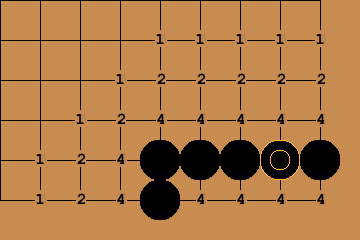
\includegraphics[width=\textwidth]{heur/4a.png}
\caption{Value is halfed each step away from the key group}
\label{fig:heur-4a}
\end{subfigure}\qquad
\begin{subfigure}[b]{0.35\textwidth}
\centering
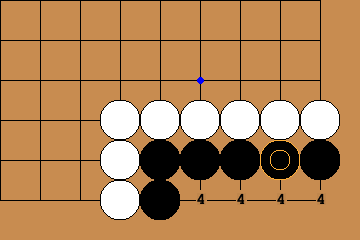
\includegraphics[width=\textwidth]{heur/4b.png}
\caption{White stones devalues moves outside the wall}
\label{fig:heur-4b}
\end{subfigure}
\caption{Distance Based Relevancy}
\label{fig:heur-4}
\end{figure}

One heuristic used to process the current board is a simple distance-based method. It relies on the school of thought that the closer a move is to the key group of stones the higher relevancy they have. Within Go-LD, the search is aware of the key group of stones (marked by keystones) hence the distance-based heuristic will give a high relevancy score to any moves one step away from the key group then a lesser score to moves two steps away and so forth. This process is used for moves up to three steps away from the key group as the relevancy of moves further away is minuscule and hence a waste of time to process. This heuristic also accounts for enemy stones which are blocking the key group's access to other points hence in situations like the one in ~\autoref{fig:heur-4b} where points that are blocked by the surrounding white stones are considered irrelevant.



The other heuristic method used for move generation is based on pattern matching. Similar to pattern matching for board evaluation, here we use pattern matching to identify relevant moves. The same patterns used for board evaluations are also used to identify relevant moves on the board. The move generator searches for patterns on the board and increments the relevancy score to any moves which are vital points within a pattern found. This will allow the move generator to consider more complex shapes on the board and generate moves according to these shapes. In general, moves found through pattern matching are given higher relevancy score than ones found through the distance-based heuristic. The flaw in this heuristic is of course only a limited number of patterns can be searched because increasing the number of patterns will increase time taken to generate moves hence the same crucial patterns used for board evaluation are used for the move generator.

\begin{figure}[!ht]
\centering
\begin{subfigure}[b]{0.35\textwidth}
\centering
\includegraphics[width=\textwidth]{heur/5a.png}
\caption{Not surrounded by white stones}
\label{fig:heur-5a}
\end{subfigure}\qquad
\begin{subfigure}[b]{0.35\textwidth}
\centering
\includegraphics[width=\textwidth]{heur/5b.png}
\caption{Surrounded by white stones}
\label{fig:heur-5b}
\end{subfigure}
\caption{Distance \& Pattern Based Relevancy Combined}
\label{fig:heur-5}
\end{figure}


Relevancy score from the distance-based heuristic and pattern-based heuristic are combined together for each valid move and is ordered into a list from the highest to the lowest relevancy.  Depending on the user’s choice of breadth limit x,  the top x number of moves from this list will be generated and used  within the search.~\autoref{fig:heur-5} shows the same board positions shown in  ~\autoref{fig:heur-4} but with both distance-based and pattern-based heuristic applied. We can see that relevancy value for the vital points of the key group is significantly higher than all the other points nearby. The move generator would pick the two vital points as the first two moves to generate which is the best case scenario for the move generator.



% \subsection{Suicidal Move Removal}
% Keystones are the absolute objective in a problem, they are one of the reference points which the tree search checks to see if the problem is solved or not. From the defender’s perspective, any moves that are detrimental to the immediate safety of the keystones needs to be removed from the list of valid moves to be searched. That entails removing any suicidal moves that decrease the number of liberties of a keystring to one.
%
% The program uses the fact that placing one stone can at maximum remove one liberty of a keystring to identify the moves which need to be removed from the moves list. Go-LD only needs to look at the moves that place a stone in liberties of keystrings with two liberties; any more liberties would ensure at least two liberties would remain intact if a stone were to be placed on a liberty. For a keystring with two liberties, placing in one of those two liberties does not automatically mean it is a suicidal move for two reasons: Move captures an opponent string; Move would increase or maintain the liberty count. If any of these two reasons are met, then the move is not suicidal. Note that "suicidal move" referred in this section is not the same as a self-capture move but rather it is a move which will lead to the opponent winning next turn.
% The following steps are used to determine the “suicidal moves” to remove from the moves list. The steps are performed on keystrings with only two liberties.
% \begin{itemize}
%     \item Both liberties of the keystring is added to the suicidal move list.
%     \item Moves that places a stone in the liberty of any opponent string which is in Atari is removed from the suicidal move list.
%     \item Moves that connects the keystring to another string which fits the following criteria are removed from the suicidal move list: Must be the same colour as the keystring; Has more than 2 liberties or has 2 liberties which are not the same 2 liberties of the keystring.
%     \item Moves that places a stone adjacent to any empty point which is not a liberty of the keystring are removed from the suicidal move list.
% \end{itemize}
%
% After these steps are performed on all keystrings with two only two liberties, any moves remaining in the suicidal moves list are removed from the valid moves list – this new list of moves is referred to as the good moves list. The good moves list is used during Alpha-Beta search instead of valid moves list to save time by not searching valid moves which would lead to immediate capture of keystones. If no moves are considered “good” then the defending player is to pass instead of making a suicidal move during Alpha-Beta search.




\subsection{Bad Move Removal}
To limit the search space, the "bad move" removal removes any moves from the defender's side which helps the attacker win the next turn — removing any moves which would decrease the number of liberties for keystring from two to one.

Placing a stone can at maximum decrease a keystring's liberty by one hence only keystrings with two liberties are checked via the following procedure. The following steps are used to determine the "bad moves” to remove from the moves list. The steps are performed on every keystrings with only two liberties.

\begin{itemize}
    \item Both liberties of the keystring are added to the "bad moves" list.
    \item Moves that capture opponent stones (i.e. play on opponent group's last liberty) are removed from the "bad moves" list.
    \item Moves that connect the keystring to another string of the same colour which has more than two liberties or has two new liberties are removed from the "bad moves" list.
    \item Moves that place a stone adjacent to any empty point which is not already a liberty of the keystring are removed from the "bad moves" list.
\end{itemize}

After, any moves remaining in the "bad moves" list are removed from the valid moves list. The remaining moves list is used during the Alpha-Beta search. If no moves remain in the moves list, then the defending player is to pass instead of making a "bad move" during the search.














\chapter{Implementation}
This chapter will go into detail about Go-LD's implementation. Go-LD is entirely written in Java and uses a simple 2D game engine called  \cite{SLICK2D} based on  \cite{LWJGL}. All of the major constructs of Go are implemented within Go-LD to create a stable environment for the user to solve Life and Death problems.  The Go board and the pattern matcher are two key aspects of Go-LD. The Go board is essentially the entire backbone of the program required to either play the problems or to create them. The pattern matcher is used to implement heuristics for both board evaluation and move generation.

\section{Board}

The Go board is represented as an object class within Go-LD which contains all the vital data to represent the current board position. Go-LD's board is designed to make the tree search and board evaluations as quick as possible. To do so meant storing more information within the Board object was ideal instead of recalculating information every time it was needed during board evaluation or move generation. The Board object also implements public methods which allow the computer and also the user to interact with the board. The rules of Go are implemented via the Board object which automatically checks if a move played by the user or the computer is valid. If it is valid then the board position is updated to represent the result of the move played otherwise if the move is invalid the Board object denies the move and creates an in-game message to let the user know.

\subsection{Stones}
Representation of stones on the board is simple but sufficient to keep the operation of gathering information about stone strings and liberties fast. Go-LD takes advantage of Java’s enum type to define the different possible states each intersection on the board could be. While it is possible to represent all the points on the board with merely black, white or empty constants, this would lead to additional operations to distinguish between different types of points such as an empty intersection which is within a problem’s boundaries and an empty intersection which is removed from play. Similar operations are required to distinguish between Ko points and Valid points, black stones and key black stones, white stones and key white stones. To avoid this problem, Go-LD uses seven different constants to represent all the intersections on the board. The "Stone" enum class consists of the following constants: BLACK, WHITE, VALID, INVALID, KO, BLACKKEYSTONE, WHITEKEYSTONE .

The entire board is represented by a 2D array of the "Stone" objects. While the use of a 1D array is possible to represent a 2D Go board and is more space efficient than a 2D array, it would require additional operations to define the board within a 2D coordinate system. This would lead to an additional operation each time the board is accessed which would slow down the entire program.

\subsection{Strings}
A string of stones is any number of stones of the same colour which are connected through adjacent stones of the same colour. A key observation of strings is that once a string is formed, the only way to deform it is through capture by placing on all the liberties of the string. Hence the Board object maintains two collections of strings, one for black and one for white, for the use of the capture functionality. Both collections of strings are updated after each move to represent any changes on the board. A list of 2D coordinates represents each string, due to the lack of an inbuilt tuple type with Java, Go-LD uses a custom-built Tuple object to represent 2D coordinates.

\subsection{Capture}
The two collections of strings stored within the Board object are used to check for capture. First, the opponent's collection of strings are checked to determine whether any opponent string lack liberties. If there is an opponent string which does not have any liberties, then it is captured. After the opponent's collection is checked, the current player's strings are also checked to keep the integrity of the board. If an opponent string has zero liberties, then every stone in the string is replaced by a VALID in the 2D array, and the string itself is removed from the collection of opponent strings. The same is applied for current player's strings but if capture occurs the move is invalidated under the self-capture rule.

During this process, two additional information is gathered about the board. Any opponent string with one liberty is considered to be in Atari and hence the intersection of the one liberty is added on to the opponent’s Atari list which consists all of the opponent’s single liberties and the same applies for the current player's strings. The two Atari list, one for each colour, is maintained within the Board object and is updated during the process of checking for capture.

The other additional information gathered is whether or not the Ko rule should be in play the next turn. While checking the opponent’s strings for capture, if a string containing only one stone is captured then the intersection of that one stone is in consideration for Ko. After checking for capture, a simple test for Ko is performed. If there is an intersection in considerable for Ko, then the stone placed this turn is checked for the following:

\begin{itemize}
    \item Does the stone only have one liberty?
    \item Is the stone by itself (not connected to adjacent stone of the same colour)?
    \item Is the liberty of the stone in consideration for Ko?
\end{itemize}

If true for all three questions, then a KO is placed inside the 2D array at the intersection which was in consideration for Ko. Next turn, the opponent cannot play there.

\subsection{Valid Move Checker}
Valid move checker is a simple function which returns true or false depending on whether placing on the intersection being checked is valid for the current player. This function consists of three core checks. Is the point being checked on the board? In case of a human player trying to place a stone outside the board grid area. Is the value of that intersection in the board’s 2D array VALID? This restricts the user and the computer from playing on points of the board which are removed from play during a problem represented by INVALID and also restricts play on the point of KO. The third check is to make sure that if the current player plays on the point, it will not lead to self-capture. The self-capture check is quite intricate, the following algorithm is used to determine whether a move is considered self-capture hence invalid.

\begin{algorithm}[H]
\caption{Self-Capture Check}\label{Self-Capture Check}
    \DontPrintSemicolon
    \SetKwFunction{FselfCapture}{selfCapture}
    \SetKwProg{Pn}{Procedure}{:}{}
    \Pn{\FselfCapture{$point$}}{
       \uIf{enemyAtariList.contains(point)}{$\KwRet { true}\;$}
        $ adjacents \gets getAdjancentPoints(point)$\;

        \eIf {(selfAtariList.contains(point))}{
        	\ForEach{adjacent in adjacents}{
        		\uIf{(adjacent is currentColour)}{
        			$adjancentString \gets getString(adjacentPoint)$\;
        			\lIf{($getLiberties(adjacentString).size > 1$)} {$\KwRet { false}\;$}
        		}
        		\ElseIf{(adjacent point is empty)}{$\KwRet { false}\;$}
        	}
    	    {$\KwRet { true}\;$}
	    }{
    	    \ForEach {(adjacent in adjacents)}{
    		    \uIf{(adjacent not enemyColour)} {$\KwRet { false}\;$}
    	    }
    	    {$\KwRet { true}\;$}
	    }
    }
\end{algorithm}

The valid move checker is integral during the tree search. Every time the search visits a new board position, the Alpha-Beta algorithm requires the list of all valid moves to generate moves using the move generator and then continue the search by trying out the generated moves. To create the list of all valid moves the valid move checker checks every point on the board, and if a point is valid, then it is added on to the list of valid moves. To reduce redundant processing, the valid moves list is maintained within the Board object and is only updated after every move.

\section{Pattern Matcher}
The pattern matcher within Go-LD can identify a pattern at the 16 possible variations which can occur. A pattern can be rotated at 45° on the board to create eight different rotations of the same pattern, and each pattern can have the colours as normal or inverted hence 16 variations. Specific to the Go board some points are regarded differently to other points, and hence the pattern matcher should be able to distinguish between these. The pattern matcher within Go-LD can define and identify patterns which are on the side, corner or the middle of the board.

\subsection{Defining Patterns}
Go-LD uses a limited number of predefined patterns which are used within its heuristic pattern matching functions. These predefined patterns are written in simple text notations which are all translated into lists of “Point” objects during the initialisation of static variables. A pattern is just a list of Point objects, and these Points are the key components the pattern matcher uses to identify patterns on the board. A Point consists of few fields which allows the pattern matcher to relate each Point to another within a pattern. These fields include two integers which can relate each Point inside the pattern to the starting point of the search in terms of distance. The other fields include boolean variables to check whether a Point is on the side, is on the corner, is defending colour or whether it is a wildcard (always matches). The text notation which is used to translate a string to a list of Points representing a pattern uses each of the characters in the string to create a Point object. ~\autoref{fig:pat-1} shows a Bent Four Corner pattern represented by text notation and the visual representation of the pattern within Go-LD. Note here the green stone marked with C shows that the pattern requires that point to be a corner point.

\begin{figure}[!ht]
\centering
\begin{subfigure}[b]{0.2\textwidth}
\includegraphics[width=\textwidth]{pat/1.png}
\caption{“xrxldxdxlxdxrr\#”}
\label{fig:pat-1a}
\end{subfigure}
\caption{Visual representation of a pattern}
\label{fig:pat-1}
\end{figure}

\subsection{Matching Patterns}

The patterns matcher itself is based on the idea that every Point object within the pattern is relative x, y distance from the starting point of search. Hence the pattern matcher always deems the starting point as x and y = 0 for the purpose of pattern matching and then it will search for the rest of the pattern relative to this starting point, a starting point is also required to contain a stone. The pattern matcher depends on three parameters, the list of Point object which represents the pattern to look for, a list of intersections all containing stones used as starting points for the pattern matcher and the colour of the defending team. Simple pseudocode for the pattern matching algorithm utilised before some additional enhancements is shown below.

\begin{algorithm}[H]
\caption{Pattern Matcher}\label{Pattern Matcher}
    \DontPrintSemicolon
    \SetKwFunction{FmatchPattern}{matchPattern}
    \SetKwProg{Pn}{Procedure}{:}{}
    \Pn{\FmatchPattern{$startingPoints,pattern,defColour$}}{
        $matches \gets$ {init list of Tuple lists }\;
        $rotations \gets$ {init list of 8 rotations}\;

        \ForEach{$stuple$ in $startingPoints$}{
            $ matchTries   \gets$ {init list of 8 Tuple lists}\;
            $ skipList  \gets$ {init list of 8 booleans initialised false}\;
            \ForEach{$Point$ in  $pattern$}{
                \lIf{(skipList.allEquals(true))} {$break$}
                 $ checkingTuple \gets$ {$stuple + (Point.x,Point.y)$}\;
                 \ForEach{$rot$ in $rotations$}{
                    \lIf{(skipList[rot]=true)}{break}
                    $ t \gets$ {$checkingTuple.apply(rot)$}\;
                    \uIf{Point.matches(t,defColour)}{
                        $matchTries$.get(rot).add(t)\;
                    }\Else{
                        $skipList[rot] \gets true$\;
                    }

                 }
            }
            \ForEach{$tupleList$ in $matchTries$}{
                \uIf{(TupleList.size() = pattern.size() \textbf{and} !matches.contain(TupleList))}{
                    matches.add(TupleList)
                }

            }

        {$\KwRet { }matches\;$}
        }

    }
\end{algorithm}

The pattern matcher returns not only the matched patterns but also the rotation of the matched pattern. Go-LD uses the matched patterns along with its rotations to find vital points within each pattern found. Then checks if these vital points are empty, contains defending colour stones or attacking stones to evaluate the value of the overall pattern found. After which more complex checks are performed to see if the pattern identified is fully formed or incomplete, whether the walls of shape are safe or not. ~\autoref{fig:pat-2} shows Pyramid Four pattern incomplete where the vital point is not as important, next to a fully complete variation of the same shape where the vital point at \bo{a} is the only point that matters.

\begin{figure}[!ht]
\centering
\begin{subfigure}[b]{0.35\textwidth}
\centering
\includegraphics[width=\textwidth]{pat/2a.png}
\caption{Incomplete \& unsafe walls}
\label{fig:pat-2a}
\end{subfigure}\qquad
\begin{subfigure}[b]{0.35\textwidth}
\centering
\includegraphics[width=\textwidth]{pat/2b.png}
\caption{Complete \& safe walls}
\label{fig:pat-2b}
\end{subfigure}
\caption{Pyramid Four pattern with and without corner stones}
\label{fig:pat-2}
\end{figure}








\chapter{Evaluation}

This chapter covers the evaluation process of the project. Which includes evaluation of the “computer” player within Go-LD and how well it solves problems and also the evaluation of the overall program.  First, we look at how the computer handles some specific Life and Death problems which are explained in detail for the reader to understand. A set of problems solvable by the computer were used to evaluate the computer’s performance quantitatively. We also go into detail about beta-testing performed at the end of the project and review the feedback/reports received.

\section{Example Life and Death Problems}
\subsection{Problem 1}
~\autoref{fig:ep1}  shows a basic problem the computer can solve at depth 1. To begin with, let us look at what happens if black is to play the initial move. Black can only live here by playing at \bo{a} or \bo{b} otherwise optimal white play will capture the black group. If black plays at \bo{a} then white needs to play at both \bo{b} and \bo{c}.Otherwise if black play at \bo{b} the white needs to play at \bo{d} and \bo{a}. Since white cannot make two moves at once, the black group lives if played correctly. Let us assume black plays at \bo{a} then the best move possible for white to challenge black is either \bo{b} or \bo{c}.Keep in mind in a real game of Go white would avoid playing in this area once black plays at \bo{a} or \bo{b} as it becomes impossible for white to win the situation.
\begin{figure}[!ht]
\centering
\begin{subfigure}[b]{0.8\textwidth}
\includegraphics[width=\textwidth]{ep1/1.png}
\end{subfigure}
\caption{Basic Life and Death Problem}
\label{fig:ep1}
\end{figure}

~\autoref{fig:ep1-1} shows the sequence of moves which occurs when the computer plays black. We can see the computer can play out the problem as black to produce two eyes in order to keep the black keystones alive. The computer can solve the problem with both variations of white’s response.

\begin{figure}[!ht]
\centering
\begin{subfigure}[b]{\textwidth}
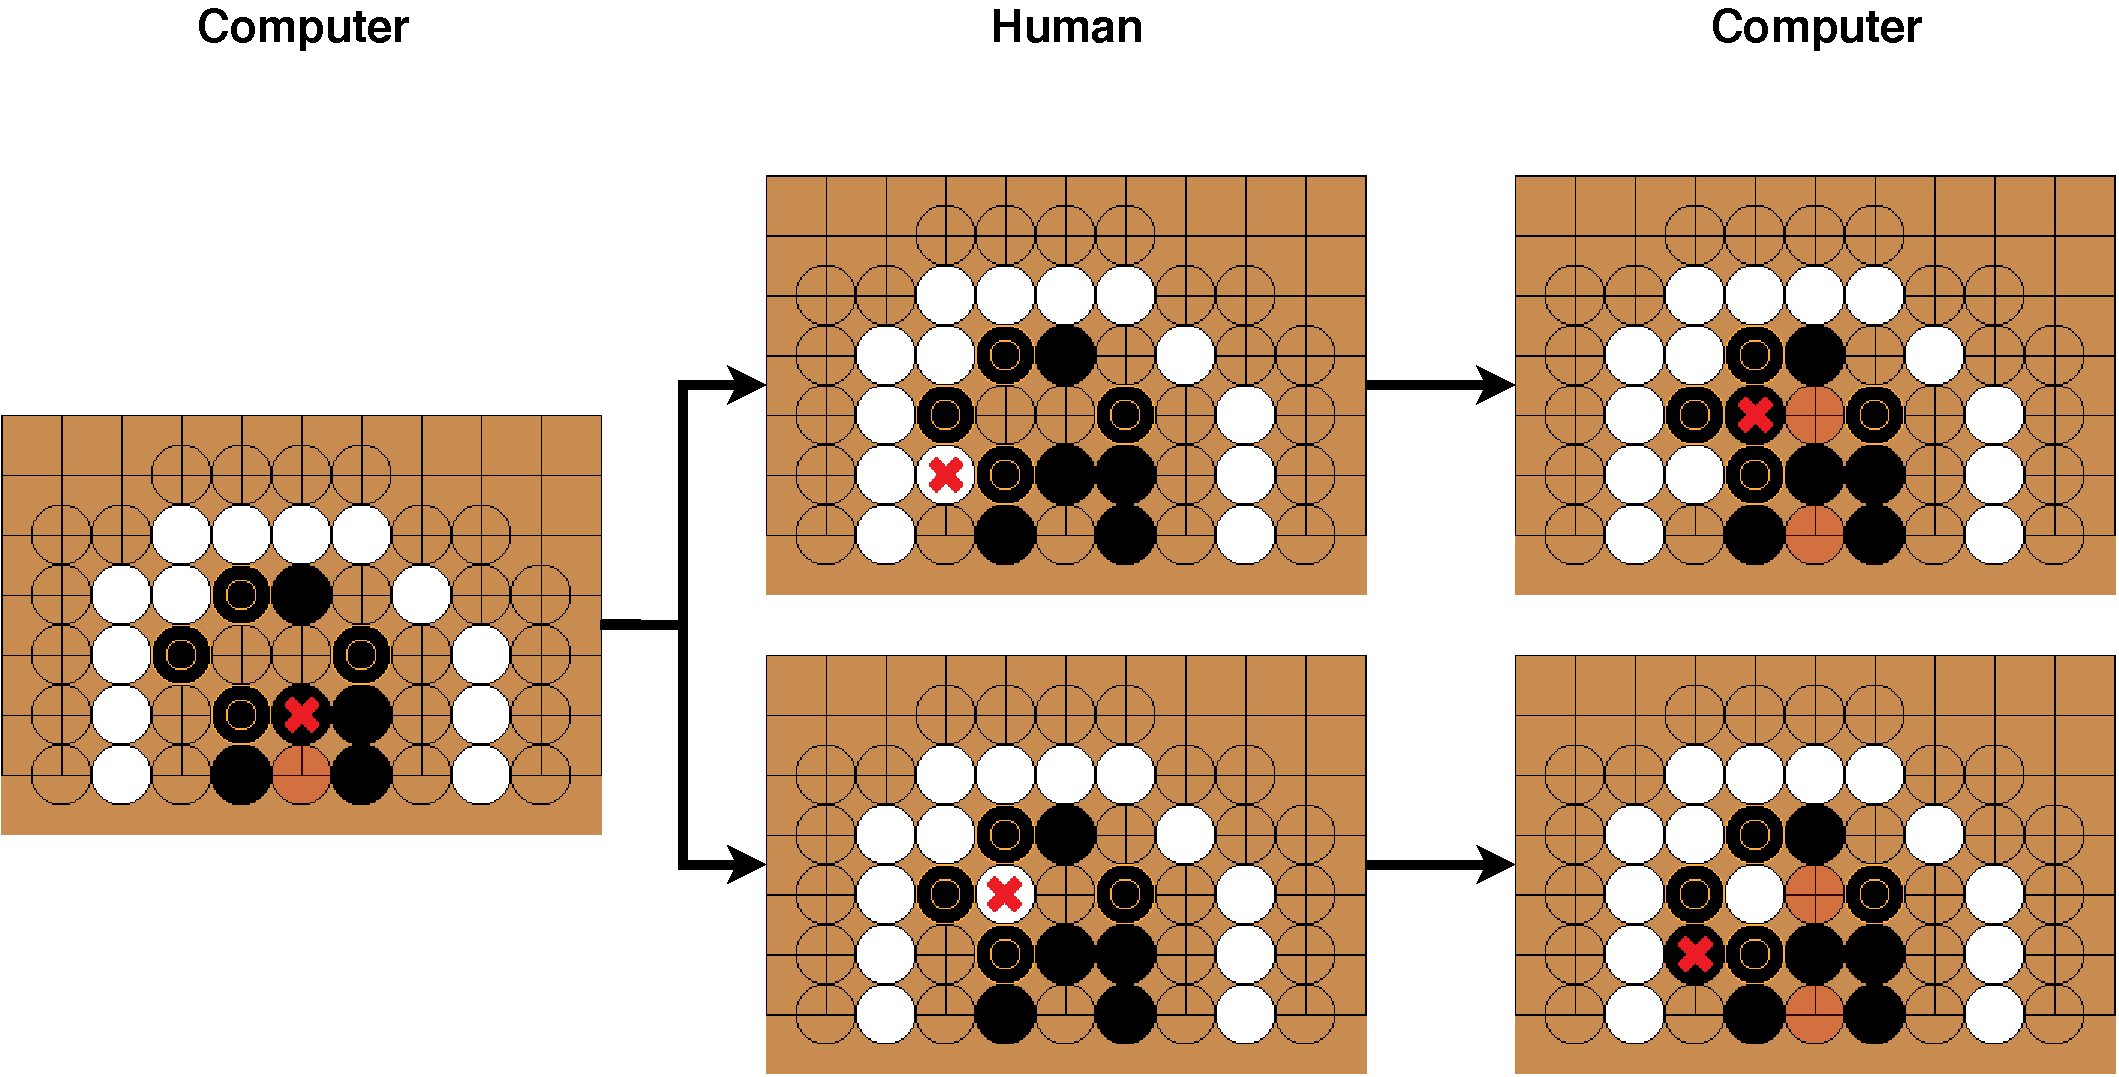
\includegraphics[width=\textwidth]{ep1/ep1-1.pdf}
\end{subfigure}
\caption{Go-LD’s “computer” solving the problem as Black first. Stone marked with x shows the move played.}
\label{fig:ep1-1}
\end{figure}

Now let us look at what happens if white is to play first. White can kill the black group in two ways. White can play at \bo{a} or \bo{b} to capture the black group. If white plays at \bo{a} then black needs to play at \bo{b} and \bo{d} to live. If white plays at \bo{b} then black needs to play at \bo{a} and \bo{c} to live. In both scenarios black needs to play at two points at the same turn which is impossible.

\begin{figure}[!ht]
\centering
\begin{subfigure}[b]{\textwidth}
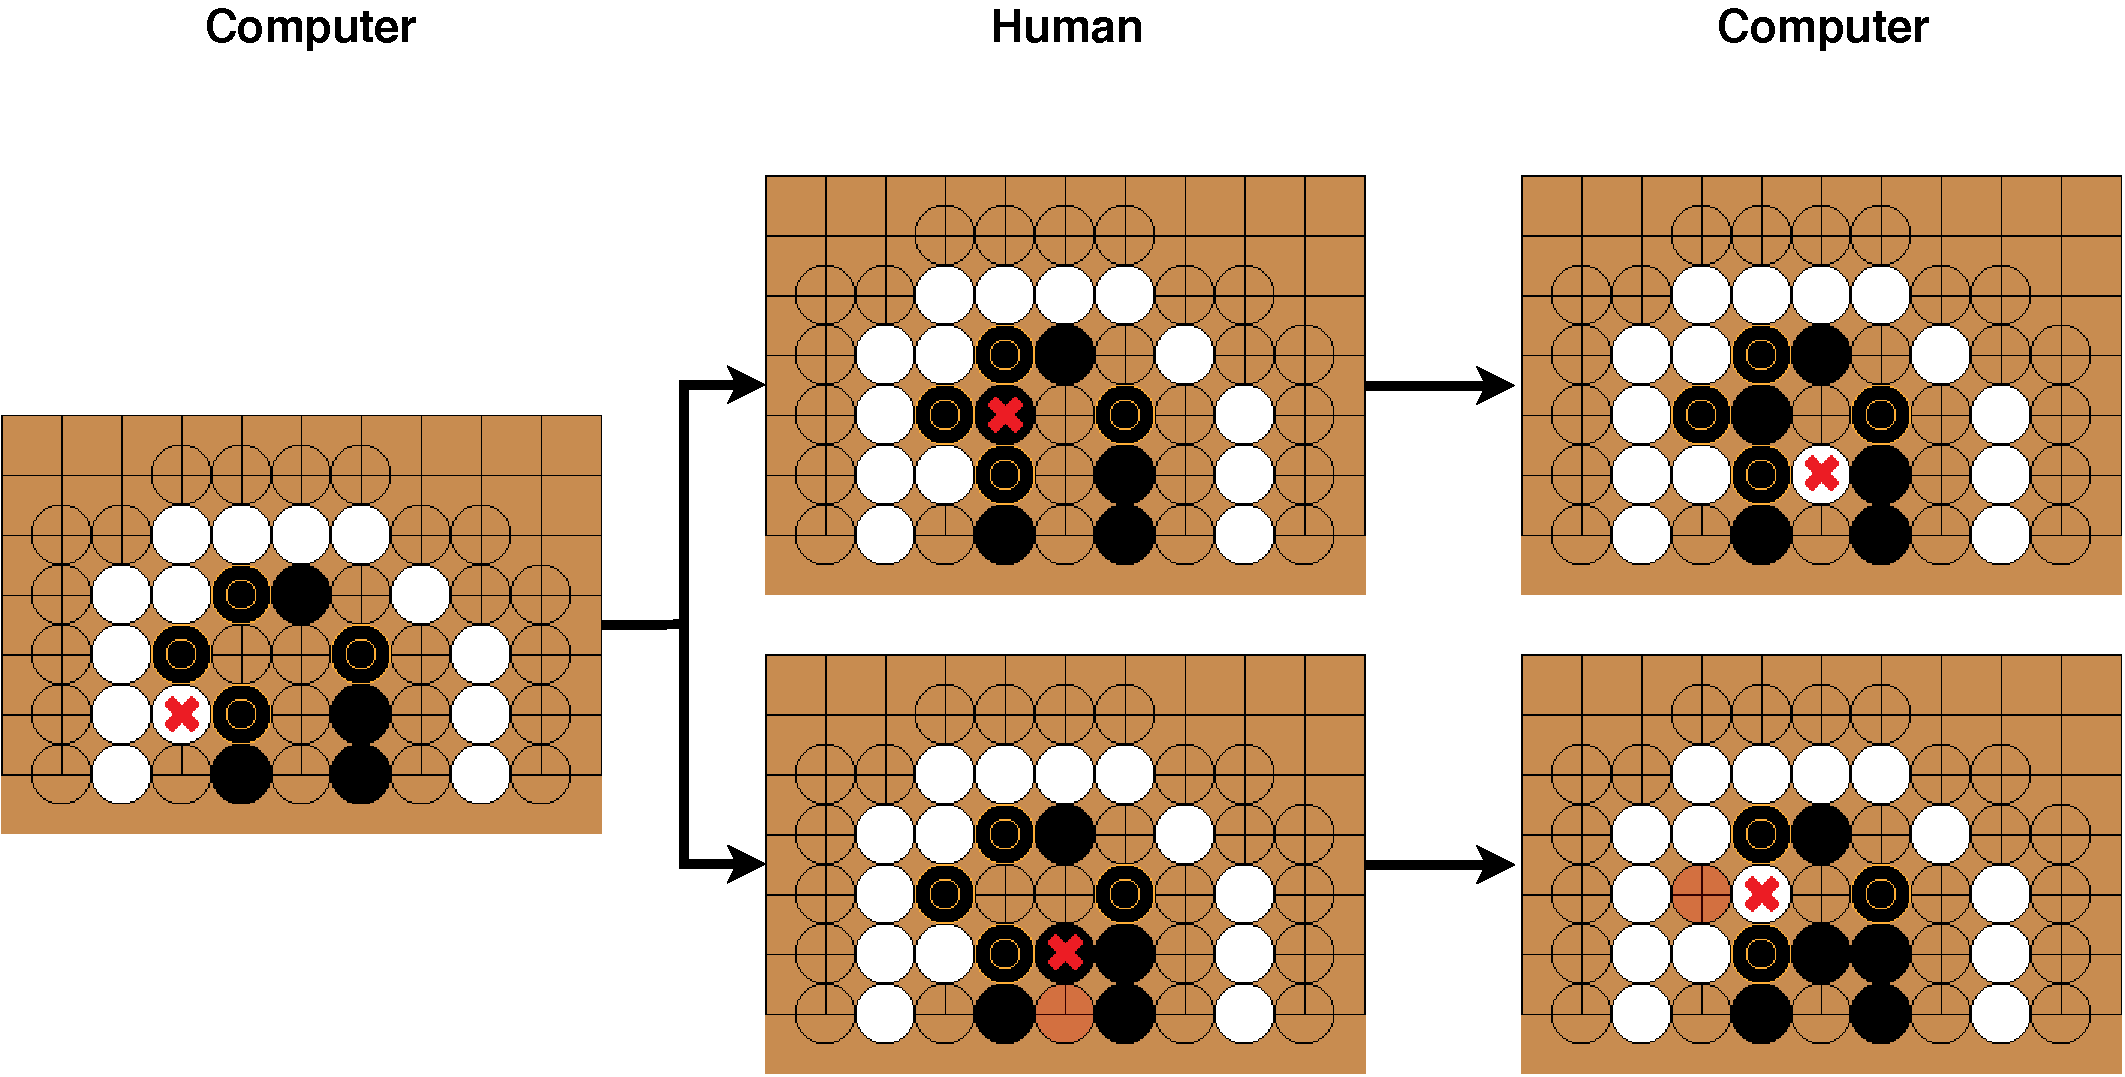
\includegraphics[width=\textwidth]{ep1/ep1-2.pdf}
\end{subfigure}
\caption{ Go-LD’s “computer” solving the problem as White first. Stone marked with x shows the move played.}
\label{fig:ep1-2}
\end{figure}


~\autoref{fig:ep1-2} shows the sequence of moves which occurs when white is to play first and controlled by the computer. The computer (white) decides to play at \bo{b} to begin. After this black has two choices, both will lead to death but will create an opportunity to live if white makes a mistake. We can see that the computer will respond correctly to both of black’s moves correctly.

\subsection{Problem 2}
~\autoref{fig:ep2} shows a more complex problem the computer can solve at depth 6. ~\autoref{fig:ep2-a} shows the sequence of moves which white should play to kill black and ~\autoref{fig:ep2-b} shows the sequence of moves black should play to live.


\begin{figure}[!ht]
\centering
\begin{subfigure}[b]{0.40\textwidth}
\centering
\includegraphics[width=\textwidth]{ep2/1a.png}
\caption{ White to kill}
\label{fig:ep2-b}
\end{subfigure}\qquad
\begin{subfigure}[b]{0.40\textwidth}
\centering
\includegraphics[width=\textwidth]{ep2/1b.png}
\caption{Black to Live }
\label{fig:ep2-a}
\end{subfigure}
\caption{Different variations depending on who plays first }
\label{fig:ep2}
\end{figure}

\begin{figure}[!ht]
\centering
\begin{subfigure}[b]{0.8\textwidth}
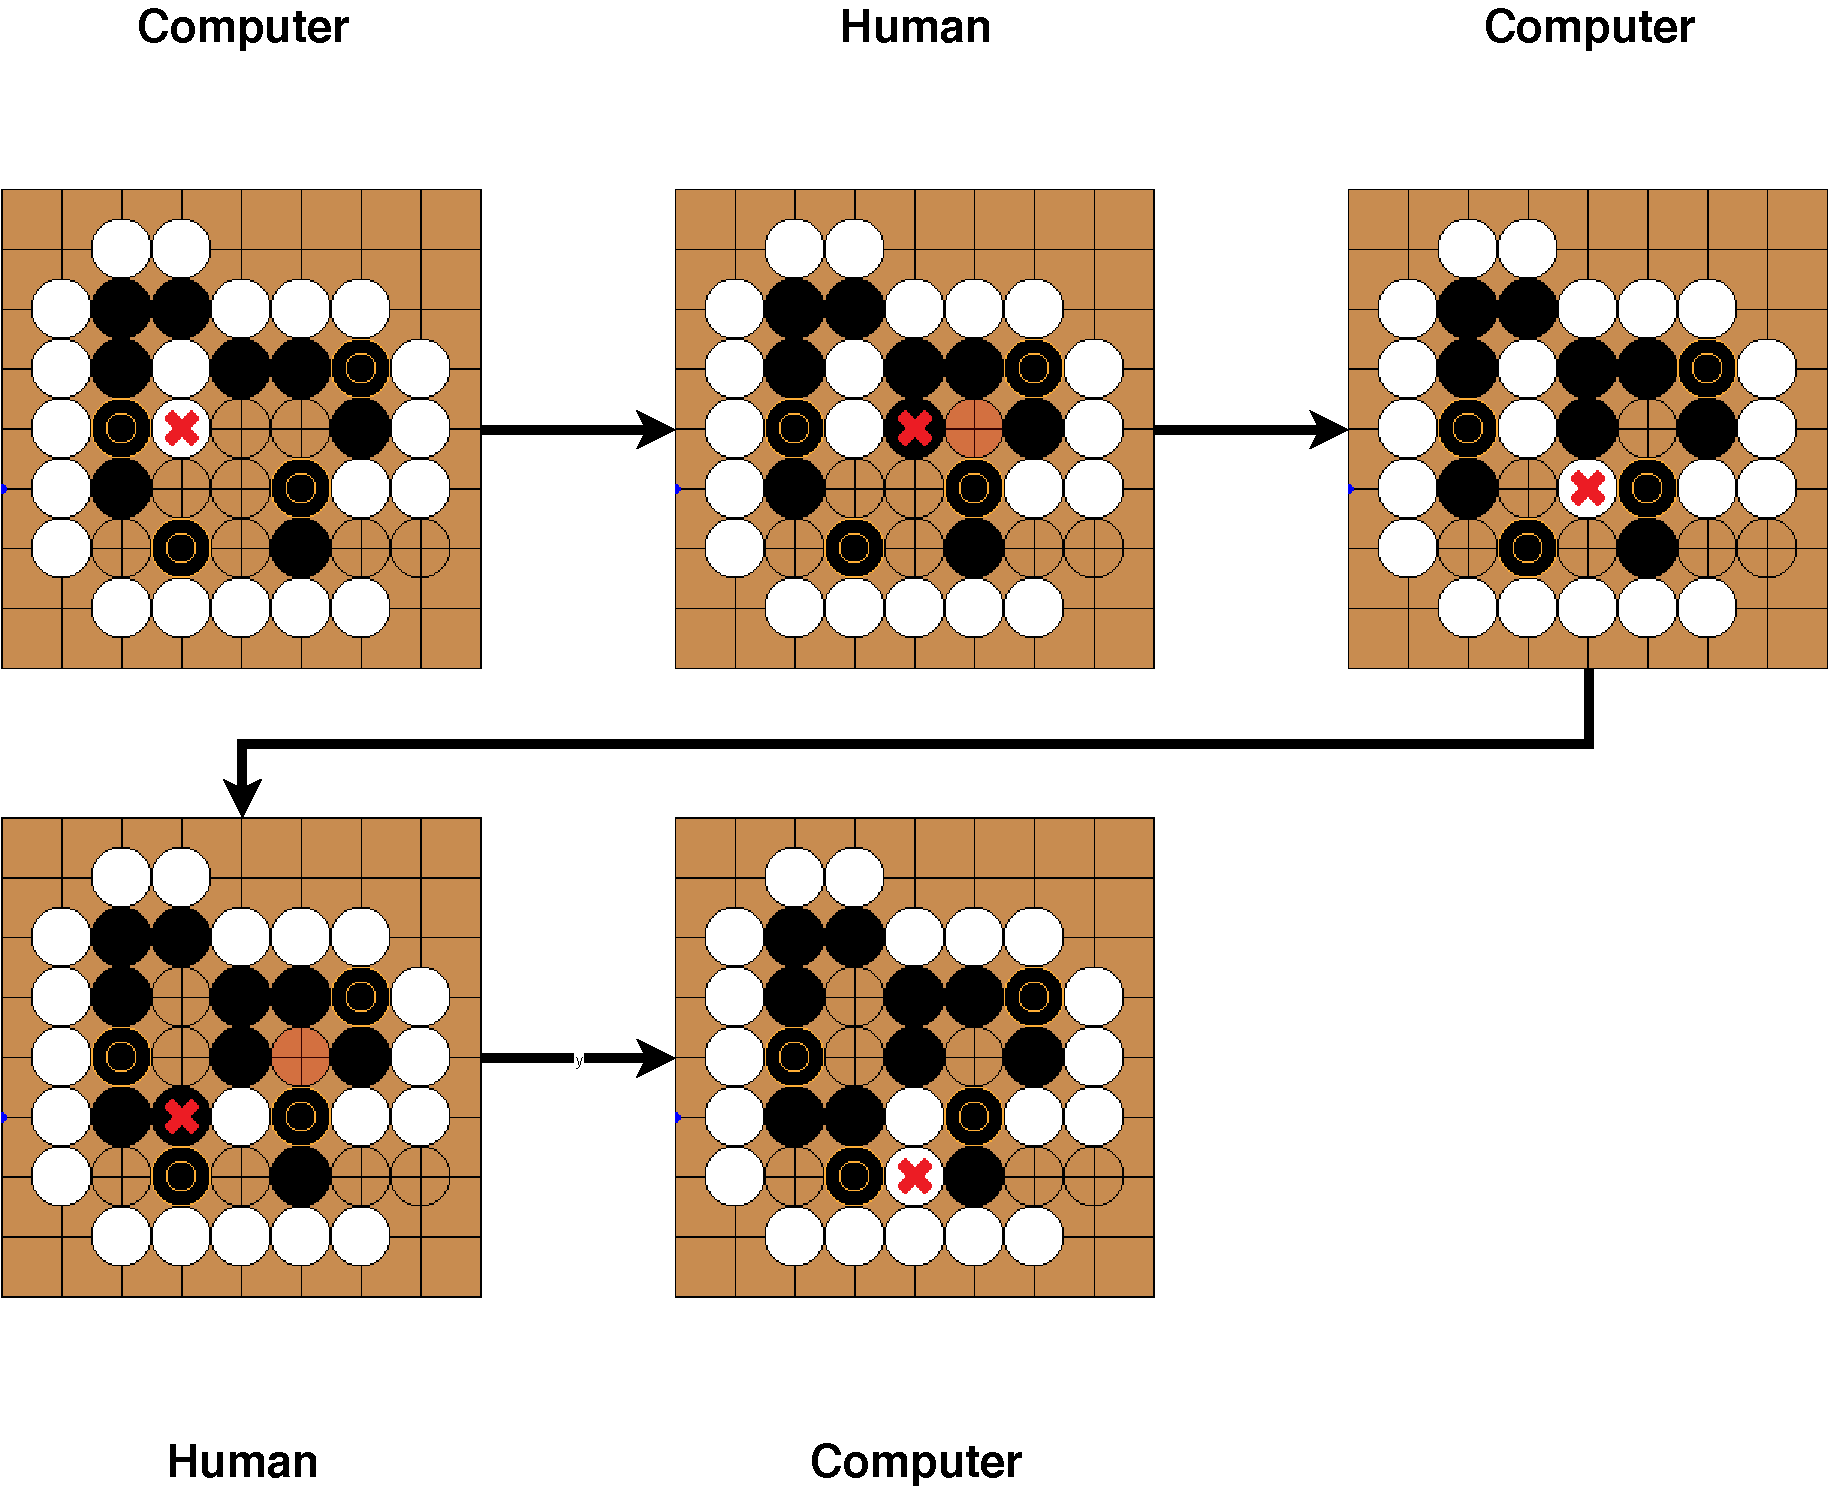
\includegraphics[width=\textwidth]{ep2/ep2-1.pdf}
\end{subfigure}
\caption{ Go-LD’s “computer” solving the problem as White first. Stone marked with x shows the move played.}
\label{fig:ep2-1}
\end{figure}


In ~\autoref{fig:ep2-1} we see the moves the computer plays as white if white were to play first and black responding in a way to maintain a chance at life. The computer figures out that playing \bo{1} is the correct move and responding to black at \bo{3} will disallow black to live. The computer kills black even if black plays its best moves.

In ~\autoref{fig:ep2-2} we can see the sequence of move the computer plays as black if black were to play first and white (human player) responding accordingly. We can see the computer provide the correct moves for black to live.

\begin{figure}[!ht]
\centering
\begin{subfigure}[b]{\textwidth}
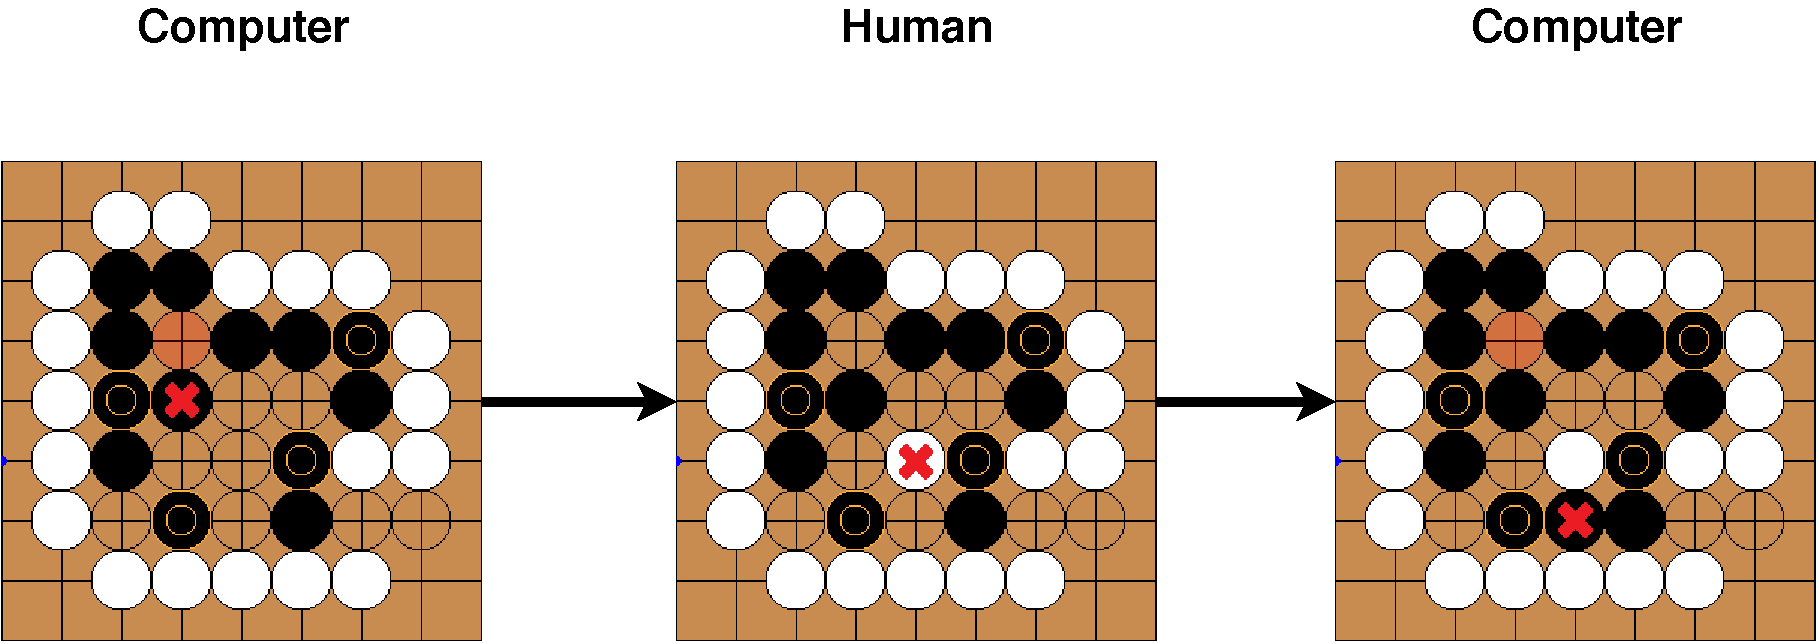
\includegraphics[width=\textwidth]{ep2/ep2-2.pdf}
\end{subfigure}
\caption{ Go-LD’s “computer” solving the problem as Black first. Stone marked with x shows the move played.}
\label{fig:ep2-2}
\end{figure}

\subsection{Problem 3}

\begin{figure}[!ht]
\centering
\begin{subfigure}[b]{0.30\textwidth}
\includegraphics[width=\textwidth]{ep3/1.png}
\end{subfigure}
\caption{2 Dan difficulty problem}
\label{fig:ep3}
\end{figure}

~\autoref{fig:ep3} shows a more complex problem than the previous examples taken from \cite{GoProblems} and is of 2 dan difficulty according to the website. Looking from white’s perspective, we can see the white group in a dangerous position. The black stone at \bo{e} reduces the eye space in the corner to 4 square points (\bo{a},\bo{b},\bo{c},\bo{d}). White can only create one real eye from this eye space because black can place a stone diagonally opposite to the point white places to disable a second eye from forming. In order for white to create two real eyes it needs to make use of the two whites stones at the \bo{f} and \bo{g} to create another eye above the white group.

~\autoref{fig:ep3-1} shows the sequence of moves which allows white to live against the optimal play from black, this is the main line of play given in GoProblems. The computer can solve this problem to win as white playing first even if black plays the optimal moves shown in ~\autoref{fig:ep3-1}. The computer is also able to solve this problem from black's perspective by playing at \bo{1} if black is supposed to play first.





\begin{figure}[!ht]
\centering
\begin{subfigure}[b]{0.70\textwidth}
\centering
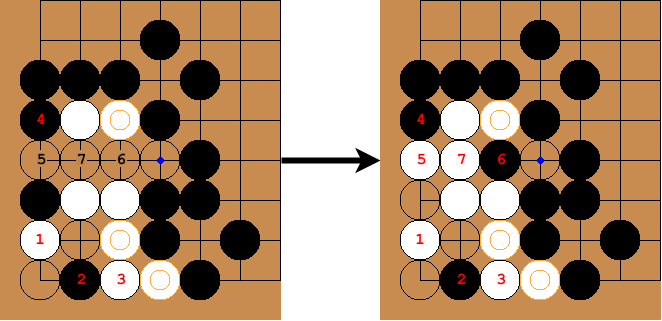
\includegraphics[width=\textwidth]{ep3/ep3-1.png}
\end{subfigure}
\caption{The sequence of moves required for white to live. Go-LD's "computer" replicates this exact sequence as white if the opponent black plays the same points.}
\label{fig:ep3-1}
\end{figure}

\section{Performance Evaluation}

The performance evaluation process for this project was executed to evaluate the speed at which the computer can find moves and the level of difficulty the computer can solve within a reasonable amount of time. Iterative Deepening was also evaluated during this process to determine if the theoretical improvement to the speed of the tree search is present within Go-LD or if Iterative Deepening decreased performance as a trade-off to give the user the ability to stop the search early.

The performance evaluation process contained the following steps:
\begin{enumerate}
\item Create a folder of Go problems from a library of problems which indicates the difficulty of each problem.
\item From this folder of Go problems, test each problem individually to determine if the problem is solvable within a reasonable time frame.
\item  Collect relevant data for every solvable problem to analyse.
\end{enumerate}

The problems used during this process were attained from \cite{GoProblems}, this website was especially helpful because it contained difficulty rating for each problem depending on how the users of the website found the problem. The reasonable time frame was two mins, but some problems were allowed slightly more time.

To determine if the computer can successfully solve a problem is a difficult task. For larger problems, it becomes impossible to test every variation of move sequences to determine if the computer can solve the problem. For this reason,  the main line of play shown on GoProblems along with some other lines of play which seemed relevant were the only ones tested. Some solution found by the computer were regarded as incorrect by GoProblems due to the difference in Ko is treated. Within Go-LD, if the attacking player can capture then they win, the occurrence of Ko does not matter whereas it does on the website.

Every problem was also tested with the objective and starting condition inverted to prove the computer is able to solve the problem from both perspectives. For example, what this means is a problem where the objective is for white to kill black and white play first then the problem is also tested with black to live and black plays first. Each problem was tested for up to 30 minutes (multiple run-throughs) to determine if it was solvable in a reasonable time frame.

The relevant data collected for each solvable problem included: The depth in which the problem is solved; The difficulty indicated on GoProblems; The identification number on GoProblems; Number of valid moves S1, S2; Four different times T1, T2, T3 and T4.

S1 – Number of valid moves with the original objective (excluding passing).

S2 – Number of valid moves with the original objective inverted (excluding passing).


T1 – Time taken for the computer to play the first move with Iterative Deepening and the original objective.

T2 – Time taken for the computer to play the first move with Iterative Deepening and the inverted objective.

T3 – Time taken for the computer to play the first move with fixed depth search and with original objective.

T4 – Time taken for the computer to play the first move with fixed depth search and with inverted objective.

In addition to these data point, each solvable problem was categorised by where they appear on the board, i.e. the middle, the sides or the corners.

\subsection{Results}
The data collected was aggregated and processed to find relevant averages and trends within it to evaluate the performance of the computer. The primary goal here was to evaluate the solving capability of the “computer” and also to find the average duration of tree search and the optimal depth parameter.

\autoref{table:extract-middle} shows an extract of data gathered from the subset of middle-based problems. Overall, data from 72 different solved problems were used, 30 for middle-based, 21 for side-based and another 21 corner-based.

\begin{table}[!ht]
\centering
\begin{tabular}{|c|c|c|c|c|c|c|c|c|c|}
\hline
\textbf{ID\#} & \textbf{Difficulty} & \textbf{\begin{tabular}[c]{@{}c@{}}Difficulty \\ Rating\end{tabular}} & \textbf{Depth} & \textbf{S1} & \textbf{S2} & \textbf{\begin{tabular}[c]{@{}c@{}}T1\\ (s)\end{tabular}} & \textbf{\begin{tabular}[c]{@{}c@{}}T2\\ (s)\end{tabular}} & \textbf{\begin{tabular}[c]{@{}c@{}}T3 \\ (s)\end{tabular}} & \textbf{\begin{tabular}[c]{@{}c@{}}T4\\ (s)\end{tabular}} \\ \hline
11650 & 12 - kyu & 1224 & 5 & 17 & 19 & 13.62 & 17.96 & 28.30 & 24.25 \\ \hline
11966 & 18 - kyu & 1047 & 5 & 11 & 12 & 3.10 & 4.10 & 3.10 & 4.52 \\ \hline
615 & 8 - kyu & 1320 & 6 & 9 & 9 & 6.89 & 7.28 & 6.11 & 4.71 \\ \hline
3206 & 7 - kyu & 1365 & 6 & 13 & 14 & 35.29 & 19.74 & 41.90 & 39.96 \\ \hline
3255 & 17 - kyu & 1064 & 6 & 14 & 14 & 15.45 & 23.59 & 34.45 & 40.72 \\ \hline
3350 & 17 - kyu & 1085 & 6 & 12 & 12 & 11.38 & 13.41 & 20.80 & 16.82 \\ \hline
3630 & 21 - kyu & 964 & 6 & 14 & 13 & 19.42 & 23.82 & 17.84 & 31.59 \\ \hline
3984 & 5 - kyu & 1412 & 6 & 11 & 11 & 25.51 & 15.40 & 26.39 & 15.94 \\ \hline
4519 & 11 - kyu & 1259 & 6 & 15 & 14 & 34.16 & 32.90 & 58.80 & 26.39 \\ \hline
4833 & 10 - kyu & 1282 & 6 & 10 & 10 & 9.25 & 6.34 & 7.91 & 4.90 \\ \hline
6219 & 8 - kyu & 1339 & 6 & 9 & 9 & 6.33 & 3.92 & 5.80 & 4.81 \\ \hline
15254 & 2 - kyu & 1508 & 6 & 8 & 8 & 2.93 & 2.20 & 1.72 & 2.50 \\ \hline
15410 & 30 - kyu & 702 & 6 & 11 & 11 & 7.81 & 9.10 & 9.97 & 12.90 \\ \hline
611 & 2 - kyu & 1495 & 7 & 9 & 9 & 12.22 & 13.23 & 11.30 & 10.55 \\ \hline
3267 & 9 - kyu & 1313 & 7 & 9 & 9 & 12.10 & 14.55 & 7.44 & 14.77 \\ \hline
% 6218 & 11 - kyu & 1240 & 7 & 10 & 10 & 30.93 & 25.69 & 29.51 & 22.60 \\ \hline
% 8626 & 12 - kyu & 1209 & 8 & 10 & 10 & 53.37 & 69.68 & 94.79 & 55.61 \\ \hline
% 15256 & 6 - dan & 1793 & 8 & 10 & 10 & 98.21 & 54.84 & 99.98 & 60.75 \\ \hline
% 16429 & 2 - dan & 1589 & 8 & 10 & 10 & 36.75 & 39.96 & 42.39 & 38.82 \\ \hline
% 7842 & 6 - kyu & 1388 & 9 & 10 & 10 & 94.64 & 62.41 & 61.42 & 19.20 \\ \hline
% 6598 & 15 - kyu & 1141 & 10 & 9 & 9 & 59.25 & 78.98 & 15.30 & 31.69 \\ \hline

\end{tabular}
\caption{Extract from the collected data for the middle-based problems subset}
\label{table:extract-middle}
\end{table}




\subsubsection{Difficulty vs. Depth}

To find the relationship between the difficulty of a problem and the depth in which it is solved at the scatter plots shown in \autoref{fig:edvd} were produced which includes the line of best fit. From the plots, we can see that increased difficulty does correlate to a linear increase in depth required. Looking at the plots we can see exceptions to this rule especially for middle-based problems, we can see instances of problems which are low in difficulty but require higher depths of search to solve. For side and corner-based problems, we find that increase in difficulty does in general results in a linear increase in depth required. We can also gather from the plots that the computer can solve difficult side-based problems at lower depths than middle or corner based ones.

\begin{figure}[!h]
\centering
\begin{subfigure}[b]{\textwidth}
\centering
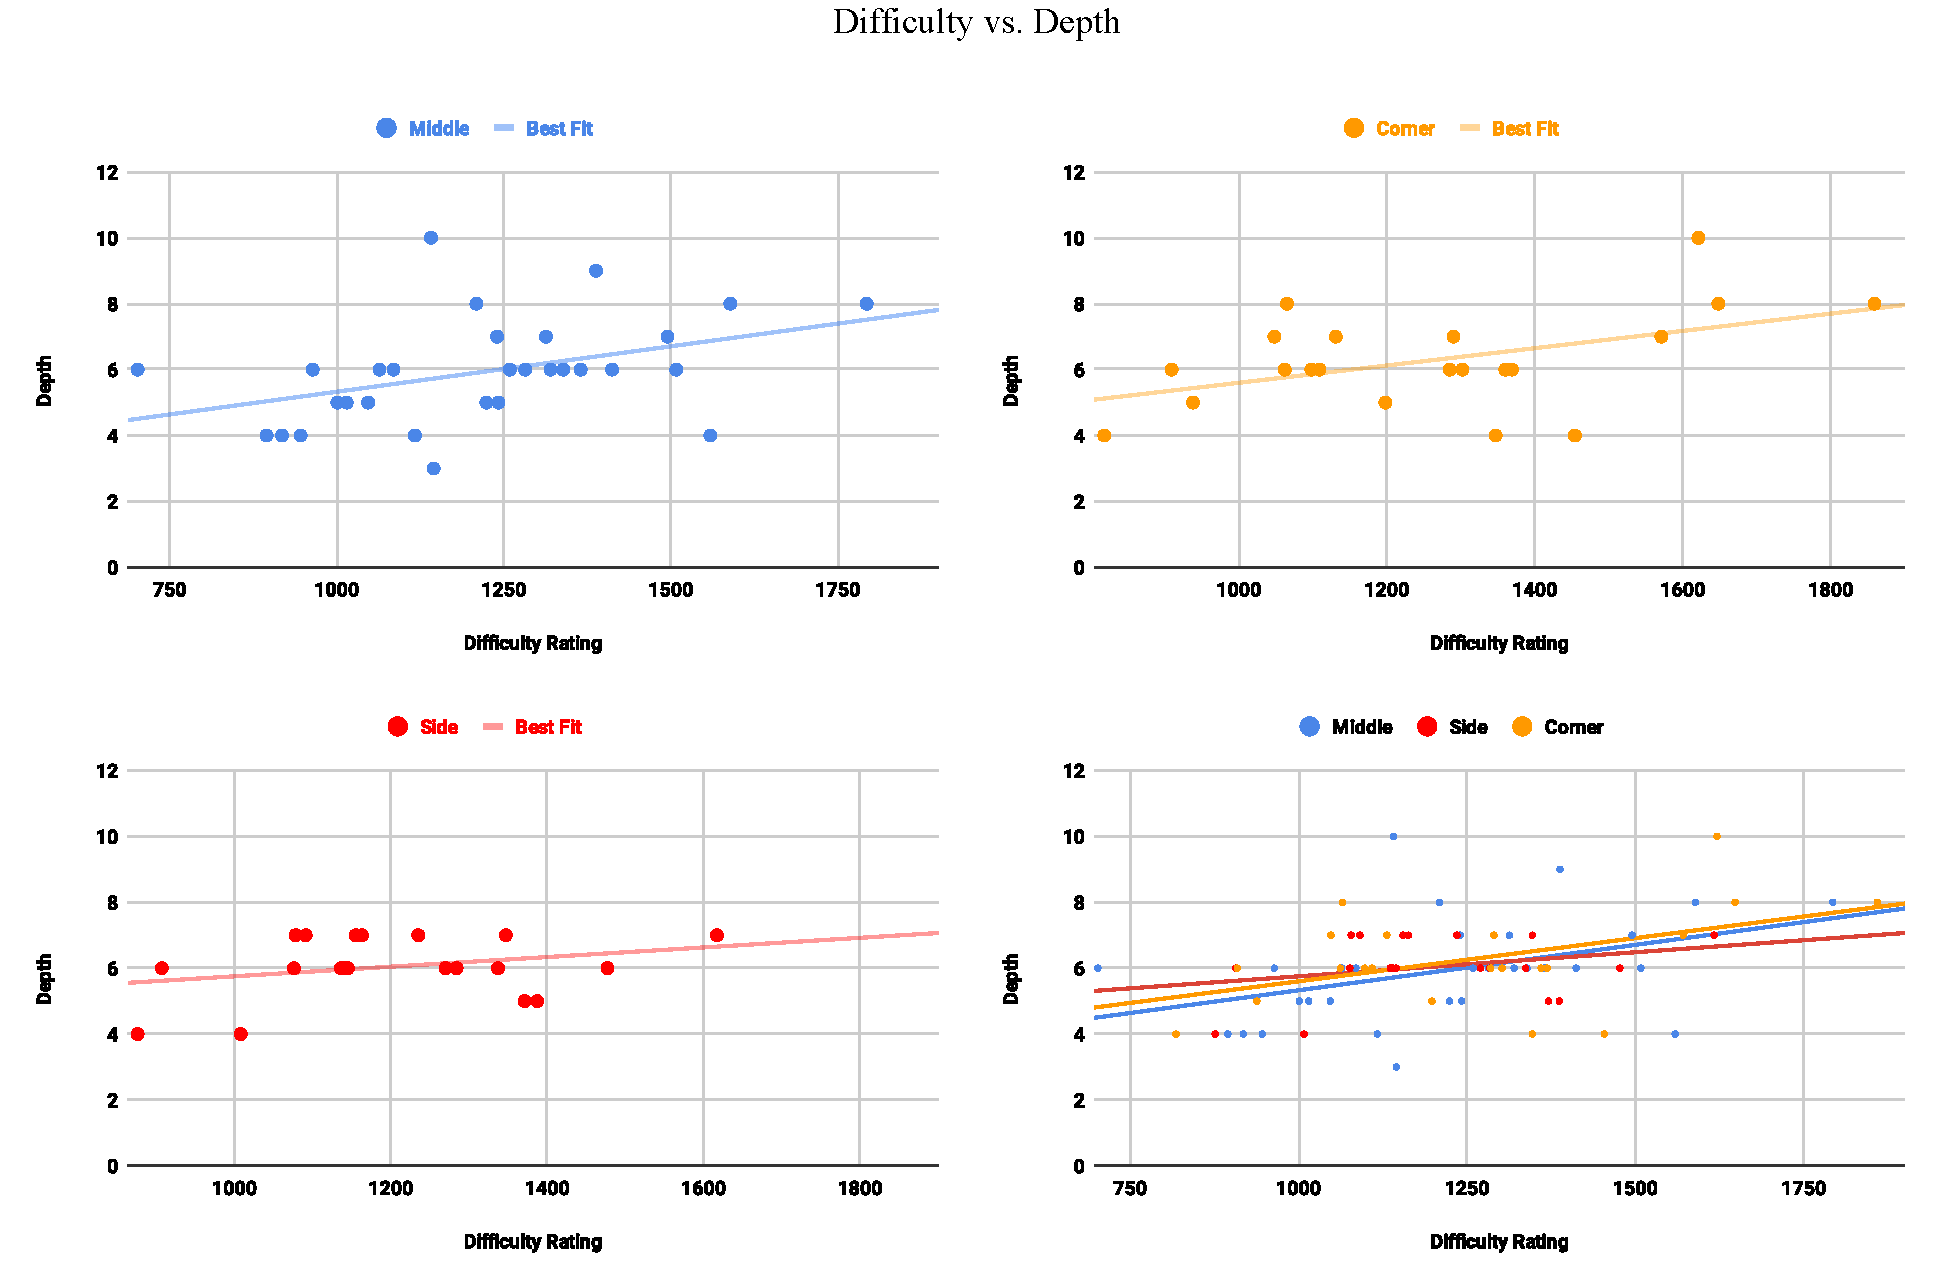
\includegraphics[width=\textwidth]{edvd/depthvdiff.pdf}
\end{subfigure}
\caption{Scatter Plots of Difficult v Depth}
\label{fig:edvd}
\end{figure}


\begin{table}[!ht]
\centering
\begin{tabular}{|c|c|c|}
\hline
\textbf{Difficulty Range} & \textbf{\begin{tabular}[c]{@{}c@{}}Difficulty Rating \\ Range\end{tabular}} & \textbf{Depth} \\ \hline
$\sim$  30 - 24 kyu  & 700 - 900 & 4.5 \\ \hline
$\sim$  24 - 16 kyu  & 900  - 1100 & 5.7 \\ \hline
$\sim$  16- 9 kyu  & 1100- 1300 & 6.2 \\ \hline
$\sim$  9 - 2 kyu & 1300 - 1500 & 6 \\ \hline
$\sim$  2 kyu - 4 dan  & 1500 - 1700 & 6.1 \\ \hline
$\sim$  4 - 7 dan & 1700 - 1900 & 8 \\ \hline
\end{tabular}
\caption{Average depth  required for varying ranges of difficulties}
\label{table:dranged}
\end{table}

\autoref{table:dranged} shows the average depth required for different ranges of difficulty ratings. The naming of the difficulty is similar to the player ranking system used in Go \citep{GoRanks}, but the actual difficulty does not precisely correlate to the skill level required to solve the problem. Using this table, we can estimate the depth parameter that Go-LD should use for a problem of difficulty x. The table also shows that the average minimum depth required to solve basic problems is around 4.5. Which is a good indication of the ability of the board evaluation function, we can see that even at lower depths the board evaluation function can accurately score the board to find the correct move for easier problems. During the testing the average problem could be solved at depth 6 therefore 6 is set to be the default depth limit for the computer.

\subsubsection{Difficulty vs.Time \& Iterative Deepening}
To evaluate Go-LD's performance in terms of difficulty versus time, we need to set a time frame which can be considered as an interactive period. Using a 45 second as the time threshold, we can estimate the average difficulty of a problem which Go-LD can solve within this threshold. The average difficulty for threshold was calculated for T1 and T3 but not T2, T4 because they used the inverted objective hence the difficulty rating shown online cannot be applied to the problem. Performing the calculation on T1 which is the time taken for the search to find the first move with Iterative Deepening resulted in an average difficulty of rating 1179 which around 13 kyu according to \cite{GoProblems}. The same calculation for T3 which is with fixed-depth search results in an average difficulty rating of 1181 also around 13 kyu.

\begin{figure}[!h]
\centering
\begin{subfigure}[b]{\textwidth}
\centering
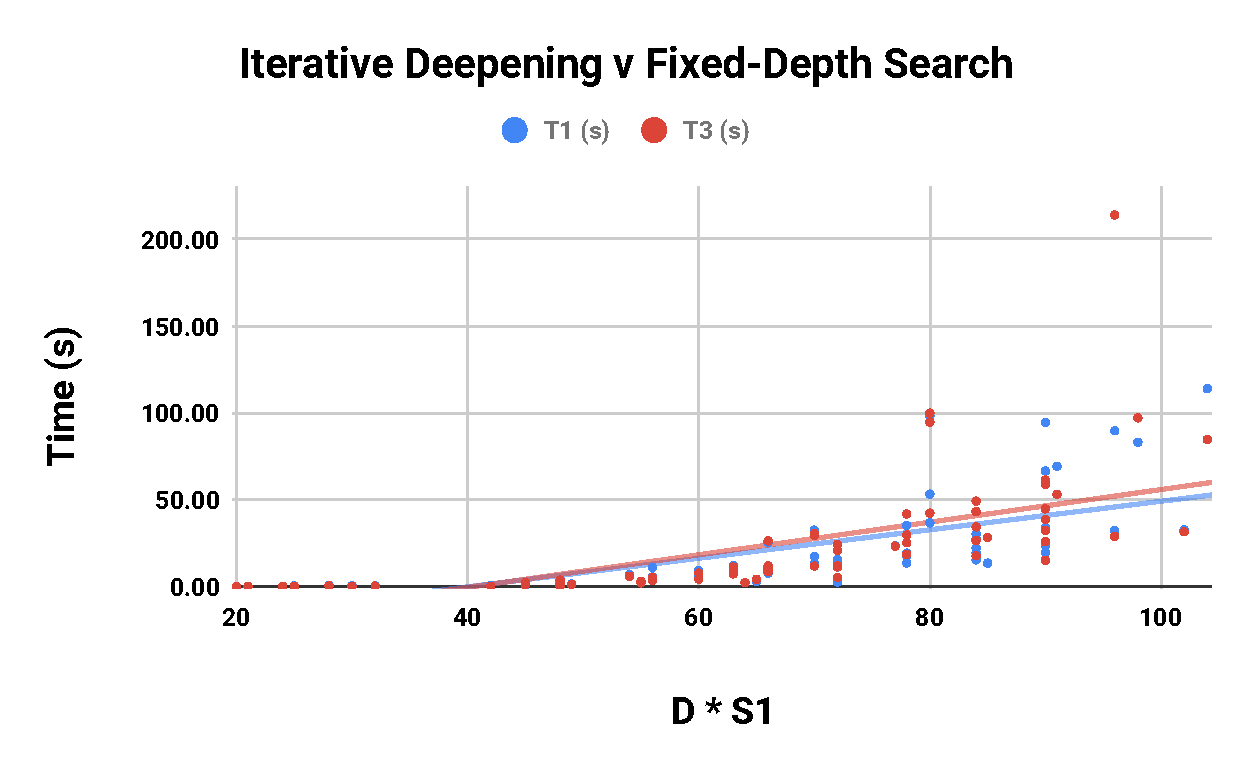
\includegraphics[width=\textwidth]{edvd/t1vt3.pdf}
\end{subfigure}
\caption{Scatter Plots of Difficult v Depth * S1}
\label{fig:t1vt3}
\end{figure}




We can look T1, T3 without setting a threshold to evaluate the addition of Iterative Deepening more clearly. \autoref{fig:t1vt3} show a plot of T1, T3 against the depth * S1 of each problem where S1 is the number of initial moves without inverting the objective. Looking at the line of best fit we can see that for shorter searches (around < 10s) the fixed depth search works better but as depth * S1 increases the more effective Iterative Deepening becomes. Note: T1 is with Iterative Deepening and T3 is fixed-depth.
\subsection{Performance Evaluation Summary}

Through the performance evaluation process, the extent of Go-LD’s “computer” player’s ability was found. Out of the 72 solvable problems gathered 18 took more than 30 seconds by the Iterative Deepening search. The remaining 54 had an average difficulty rating of 1179 (\textasciitilde 13 kyu). Iterative Deepening had a minimal negative effect for shorter searches and had a positive effect for longer searches compared the fixed-depth search. Therefore, the choice of implementing Iterative Deepening is reasonably validated as it will give users more control over the search result without hindering the performance, sometimes even improving it. This process also made the limitation of search evident; there were around 30 other problems initially re-created with Go-LD which were unable to be solved in a reasonable time frame. Most of these were of higher difficulty and larger in size than the solvable problems. This limitation was foreseen as it is the nature of heuristics, it can never be perfect and only through increased knowledge can it become more accurate. Increased knowledge requires a deeper and broader search which leads to exponential time increase.



\section{Beta Testing}
At the end of the project, the program was put forward for beta testing. The primary goal of the beta testing was to evaluate usability and functionality. A small number of beta tester were given the program for a period two weeks to test and provide feedback on different aspects of the program. They were also to report any bugs or issues found during testing. Testers were a given brief which contained an introduction to the project along with simple step by step tutorial to play through the tutorial problem provided to them. The testers also received 30 self-designed problems and the collection of 72 problems used during performance evaluation. All problems delivered to the testers contained predefined search parameters at which the computer should be able to solve the problem, and these parameters were set to load up along with the problem.

\subsection{Pre-Testing Questions}
The testers were sent a google form which they had to fill in throughout testing. To gauge the experience of the testers with Go few simple questions were asked. The results showed 4 out of the 6 testers were aware of the rules of Go, if they were not aware they were provided with a link to a simple Go rule guide to help them with the rest of the testing. Following this they were asked if they had played Go before, the result was that only 2 in 6 had played Go before and more importantly only one tester have tried solving life and death problems. A crucial take away from this is that the lack of experience playing Go within the testers would have limited the extent to which they can test the Go-LD’s computer. An inexperienced Go player might not be able to tell if the computer is playing a poor move hence will not be able to report on it.

\subsection{Interface \& Usability}
The testers were asked a series of questions regarding the interface and usability of the two modes of Go-LD (Play, Editor). Most testers agreed that the representation of the board was simple and clear, even though the testers answered this question in regard to the board in play mode it would apply for the editor mode as well because the board is represented the same for both modes.

Testers found the buttons on the play mode interface quite simple to identify. Most testers were able to distinguish between the toggleable buttons and the standard buttons. They also rated the labelling on buttons on average 4.5/5 in regard to how useful they were to identify the functionality of the button. One tester reported a lack of visual feedback on buttons and explained: “Sometimes I'm not sure if I've pressed a button or not.”

Some testers found parts of the text displayed on the screen difficult to read. One tester found the difference in font size for some buttons difficult to read and would have preferred the larger font which was already in use for bigger buttons. Another tester suggested outlining the text used on the screen would help. In terms of interactively playing through problems, all tester found that it was quite simple to place stones on the board. The testers also agreed that playing through problems were quite simple in terms of usability and the in-game messages provided were helpful.

For the editor mode interface, testers found the radio buttons to choose between which stones to place were appropriately labelled and simple to use. One tester was not able to distinguish the difference between placing a keystone and a normal stone. Which highlights a lack of visual indication for keystones but also a lack of explanation on what a keystone’s purpose is within the Go-LD and how they differ from normal stones. Testers on average found the creating problems using the editor mode and placing stones of their choice on the board relatively simple. One tester did find that placing valid points one by one “very tedious” and suggested addition of functionality to place an area of valid points along with the ability to place one by itself.

Testers found the background image used for Go-LD during beta testing too bright and one tester, in particular, found it “really hard on the eyes”.  Since this issue could be easily fixed the background was changed to something more suitable in opacity.

\subsection{Functionality \& Issues}
In terms of functionality, the testers provided quite insightful feedback to evaluate the program. When asked about the speed in which the computer responded with move testers had a variety of responses. Some deemed it to be very quick; one even said that they found it difficult to see where the computer had placed the stone. Other testers found that speed decreased with increased complexity of the problem. One tester in particular identified depth up to 6 was “fast enough to remain interactive”. The varied tester responses show that the computer dealing with simpler problems can be too quick for the user to see the stone placed on the board and when dealing with difficult problems requiring higher depths the user has to wait longer on the computer to make a move. These responses confirm the data showed during the performance evaluation process about the speed in which the computer solves the problem is relative to the difficulty of the problem which is only natural.
All testers combined found one instance of a Go problem provided to them not being solved at the set default depth for that problem. Apart from this instance, the computer was able to solve every problem the testers played if they let the computer play first.

The testers were asked if there were any difficulties during testing, one tester pointed out that the editor mode’s board taking priority over play mode’s board when switching between the two modes was an issue. While this is a functionality to allow a problem created on editor mode to be transferred over to play mode in retrospect having the ability to choose whether or not to transfer over the problem from one mode to another would have proved to be a better implementation of the functionality. Another tester found that it was quite difficult to judge the increase in time when adjusting the depth and breadth limits hence would have liked to have a warning of sorts to let them know the effect of increasing the limits too high.

A critical issue that occurred during the early phase of beta testing was that the testers found it difficult to run the program due to the difference in java version required to run Go-LD to the version they had installed. Since this was a significant hindrance, the issue was fixed during the beta testing phase by bundling the Java Runtime Environment required along with the entire Go-LD beta testing package. Furthermore, the portability has since been tested for on Windows 10, Ubuntu and  Fedora systems to ensure the program can simply run from the files inside the zipped folder containing the final version of Go-LD. Due to a lack of access to a Mac system, Go-LD was not tested on the Mac OS.

\subsection{Beta Testing Summary}
Beta testing was an excellent opportunity to understand how the software tool would perform in the hands of inexperienced users. To begin with the positives, users found the program itself pretty simple granted a tutorial was provided to them which mostly focused on introducing the testers to the basic concept of a Life and Death problems more than the whole program itself. In terms of the reliability of the program, there were no issues reported by the testers, no major bugs or crashes were reported. Go-LD could be said to be adequate in terms of performance (of the "computer") from the tester’s responses. Tester found that simpler problems could be solved quickly but increasing the depth higher could result in longer waiting times which is to be expected. The visual aspect of the program was overall the weakest point; testers reported two significant concerns, text readability and the background image. Due to the simplicity of these issues, they were immediately improved upon. The tester’s issues highlighted the visual aspects of the program which requires much improvement for future versions.





\chapter{Conclusion}

\section{Summary}
During this project, the aim of creating a software tool for Go players to create and solve Life and Death problems interactively has been achieved. The final tool written in Java has met most if not all the functional requirements put forth at the begin of the project and also the ones added during the period of the project. In terms of software engineering it was the right decision to split the entire development phase into two achievable milestones to ensure there was a clear goal at each stage of the development process.

The first milestone was to implement the main structure of the overall software tool, which included creating all the functionalities required to allow users to play through a Go problem against a computer that did not use any heuristics to find the best move possible. At the end of the first milestone, the tool contained a simple Alpha-Beta search without any depth or breadth cut-offs.

The second milestone addressed the issues with the computer’s lack of heuristics. Without heuristics, larger Go problems become impossible to solve. The first significant step in achieving the milestone was to introduce user-defined depth cut-offs to the search which relied on a board evaluation function. The board evaluation function created contains pattern matching heuristics along with a simple liberty counting heuristic.

Next step was to implement move ordering techniques. The reasoning behind doing so was to drastically decrease the number of moves the Alpha-Beta search had to look through by processing moves which could potentially produce Alpha-Beta cut-offs first. The Killer Move heuristic was the first heuristic implemented to perform move ordering. At this point of the project, Iterative Deepening was also implemented to use Alpha-Beta search to give users the ability to stop the computer in the middle of a search and force it to play the best move found so far. To go along with Iterative Deepening, the Principal Variation found during each iteration was used as the first sequence of moves to be searched during the next iteration. Finally, a move generator based on pattern matching and distance from the keystones of the problem was created to enable users to restrict the number of moves the computer searches each ply of the game tree.






Once both these milestones were achieved Go problems were created from scratch or re-created from external sources such as \cite{Cho1993}, \cite{Davies1975}, \cite{GoProblems}. The problems were created to initially test and evaluate Go-LD and then to produce a folder of problems which could be solved by the computer to be packaged along with the final version of Go-LD.

The evaluation process consisted of two parts, the performance evaluation process and beta testing. The relationship between the time for the computer to solve a problem and the difficulty of the problem was discovered during the performance evaluation process. In addition to this, the average difficulty the computer could solve in a reasonable length of time was also calculated. Iterative Deepening Alpha-Beta search was compared to fixed-depth Alpha-Beta search. The results showed that Iterative Deepening is slightly slower for problems which took less than 10 seconds to solve but as the time increased Iterative Deepening became more effective and overtook the fixed-depth search in performance. Beta testing performed over two weeks was able to provide results to evaluate the usability and interface of the program. The results convey that the overall usability of the program was adequate, but certain aspects of visual design required great improvements.

\section{Future Development}
There are many features and improvements which could be looked at to progress the work done throughout this project further. Some of the suggestions made by the beta testers seemed interesting. A popular suggestion was to add a hint button which could show the user a few good moves determined by the computer searching in the background. Another great idea was to visualise which moves the computer is considering during the search; this would mean to show the current best move according to the latest iteration of Alpha-Beta completed.

The nature of heuristics means that they are not perfect, hence looking at new methodologies to perform board evaluation, move generation and move ordering would be an ideal way to improve on what is currently in use. Specifically, some work done by B.Bouzy in his paper \citep{Bouzy2003} where he looks at improving upon the Zobrist model \citep{Zobrist1969} which is based on the idea of creating a map of influence based on the positions of stones on the board. Applying this work to Life and Death problems could help in determining which moves to generate by looking at points of high influence on the influence map. A way to improve on B.Bouzy's improved model could be by taking into consideration the difference in strength of stone patterns during the creation of an influence map. For example, four stones arranged in a square block would have a lot less influence than four stones arranged to create an eye in the middle.

Another realm of possibilities can be opened up by introducing Machine Learning to identify and group similar stone patterns to determine the value of each pattern to be used during a board evaluation function. Machine Learning could even be used to create an entirely new board evaluation function from scratch. Doing so would provide significant improvements over any human-designed evaluation function granted a large enough training set is used.







\begin{appendices}

\chapter{Performance Evaluation Data Collected}

Here is all the data collected through out the performance evaluation process. All data were collected from a computer of the following specification.

Operating System: Windows 10 Home 64-bit

Processor: AMD Ryzen 7 2700X Eight-Core Processor          (16 CPUs), ~3.7GHz

Memory: 16384MB RAM

Display Device : NVIDIA GeForce GTX 1080



\section{Middle-Based Problems}

\begin{longtable}{|c|c|c|c|c|c|c|c|c|c|}
\hline
\textbf{ID \#} & \textbf{Difficulty} & \textbf{\begin{tabular}[c]{@{}c@{}}Difficulty \\ Rating\end{tabular}} & \textbf{Depth} & \textbf{S1} & \textbf{S2} & \textbf{\begin{tabular}[c]{@{}c@{}}T1 \\ (s)\end{tabular}} & \textbf{\begin{tabular}[c]{@{}c@{}}T2 \\ (s)\end{tabular}} & \textbf{\begin{tabular}[c]{@{}c@{}}T3 \\ (s)\end{tabular}} & \textbf{\begin{tabular}[c]{@{}c@{}}T4 \\ (s)\end{tabular}} \\ \hline
\endfirsthead
%
\endhead
%
4776 & 15 - kyu & 1145 & 3 & 7 & 8 & 0.19 & 0.22 & 0.17 & 0.22 \\ \hline
5300 & 1 - dan & 1559 & 4 & 7 & 7 & 0.73 & 0.60 & 0.52 & 0.47 \\ \hline
5505 & 22 - kyu & 946 & 4 & 16 & 17 & 2.37 & 2.16 & 2.30 & 2.91 \\ \hline
7106 & 16 - kyu & 1117 & 4 & 6 & 6 & 0.26 & 0.27 & 0.18 & 0.20 \\ \hline
10491 & 24 - kyu & 895 & 4 & 6 & 6 & 0.17 & 0.24 & 0.16 & 0.13 \\ \hline
10541 & 23 - kyu & 918 & 4 & 18 & 18 & 2.73 & 2.49 & 5.24 & 4.81 \\ \hline
1384 & 19 - kyu & 1015 & 5 & 6 & 6 & 0.62 & 0.66 & 0.23 & 0.62 \\ \hline
3269 & 11 - kyu & 1242 & 5 & 13 & 13 & 3.20 & 2.89 & 4.36 & 2.64 \\ \hline
3492 & 20 - kyu & 1001 & 5 & 9 & 9 & 1.66 & 1.76 & 1.52 & 1.66 \\ \hline
11650 & 12 - kyu & 1224 & 5 & 17 & 19 & 13.62 & 17.96 & 28.30 & 24.25 \\ \hline
11966 & 18 - kyu & 1047 & 5 & 11 & 12 & 3.10 & 4.10 & 3.10 & 4.52 \\ \hline
615 & 8 - kyu & 1320 & 6 & 9 & 9 & 6.89 & 7.28 & 6.11 & 4.71 \\ \hline
3206 & 7 - kyu & 1365 & 6 & 13 & 14 & 35.29 & 19.74 & 41.90 & 39.96 \\ \hline
3255 & 17 - kyu & 1064 & 6 & 14 & 14 & 15.45 & 23.59 & 34.45 & 40.72 \\ \hline
3350 & 17 - kyu & 1085 & 6 & 12 & 12 & 11.38 & 13.41 & 20.80 & 16.82 \\ \hline
3630 & 21 - kyu & 964 & 6 & 14 & 13 & 19.42 & 23.82 & 17.84 & 31.59 \\ \hline
3984 & 5 - kyu & 1412 & 6 & 11 & 11 & 25.51 & 15.40 & 26.39 & 15.94 \\ \hline
4519 & 11 - kyu & 1259 & 6 & 15 & 14 & 34.16 & 32.90 & 58.80 & 26.39 \\ \hline
4833 & 10 - kyu & 1282 & 6 & 10 & 10 & 9.25 & 6.34 & 7.91 & 4.90 \\ \hline
6219 & 8 - kyu & 1339 & 6 & 9 & 9 & 6.33 & 3.92 & 5.80 & 4.81 \\ \hline
15254 & 2 - kyu & 1508 & 6 & 8 & 8 & 2.93 & 2.20 & 1.72 & 2.50 \\ \hline
15410 & 30 - kyu & 702 & 6 & 11 & 11 & 7.81 & 9.10 & 9.97 & 12.90 \\ \hline
611 & 2 - kyu & 1495 & 7 & 9 & 9 & 12.22 & 13.23 & 11.30 & 10.55 \\ \hline
3267 & 9 - kyu & 1313 & 7 & 9 & 9 & 12.10 & 14.55 & 7.44 & 14.77 \\ \hline
6218 & 11 - kyu & 1240 & 7 & 10 & 10 & 30.93 & 25.69 & 29.51 & 22.60 \\ \hline
8626 & 12 - kyu & 1209 & 8 & 10 & 10 & 53.37 & 69.68 & 94.79 & 55.61 \\ \hline
15256 & 6 - dan & 1793 & 8 & 10 & 10 & 98.21 & 54.84 & 99.98 & 60.75 \\ \hline
16429 & 2 - dan & 1589 & 8 & 10 & 10 & 36.75 & 39.96 & 42.39 & 38.82 \\ \hline
7842 & 6 - kyu & 1388 & 9 & 10 & 10 & 94.64 & 62.41 & 61.42 & 19.20 \\ \hline
6598 & 15 - kyu & 1141 & 10 & 9 & 9 & 59.25 & 78.98 & 15.30 & 31.69 \\ \hline
\caption{ Data collected for the middle-based problems}
\label{table:data-middle}
\end{longtable}


\section{Side-Based Problems}
\begin{longtable}{|c|c|c|c|c|c|c|c|c|c|}
\hline
\textbf{ID \#} & \textbf{Difficulty} & \textbf{\begin{tabular}[c]{@{}c@{}}Difficulty \\ Rating\end{tabular}} & \textbf{Depth} & \textbf{S1} & \textbf{S2} & \textbf{\begin{tabular}[c]{@{}c@{}}T1 \\ (s)\end{tabular}} & \textbf{\begin{tabular}[c]{@{}c@{}}T2 \\ (s)\end{tabular}} & \textbf{\begin{tabular}[c]{@{}c@{}}T3 \\ (s)\end{tabular}} & \textbf{\begin{tabular}[c]{@{}c@{}}T4 \\ (s)\end{tabular}} \\ \hline
\endfirsthead
%
\endhead
%
3153 & 19 - kyu & 1008 & 4 & 8 & 7 & 0.49 & 0.32 & 0.38 & 0.37 \\ \hline
3154 & 24 - kyu & 876 & 4 & 6 & 6 & 0.30 & 0.27 & 0.25 & 0.25 \\ \hline
689 & 7 - kyu & 1371 & 5 & 11 & 11 & 3.13 & 3.67 & 2.27 & 2.79 \\ \hline
1087 & 6 - kyu & 1387 & 5 & 5 & 6 & 0.54 & 0.20 & 0.22 & 0.06 \\ \hline
3055 & 23 - kyu & 907 & 6 & 10 & 10 & 6.39 & 4.28 & 4.35 & 2.45 \\ \hline
3138 & 10 - kyu & 1284 & 6 & 16 & 16 & 32.29 & 36.45 & 28.98 & 30.86 \\ \hline
3141 & 15 - kyu & 1136 & 6 & 13 & 13 & 17.56 & 16.65 & 25.35 & 20.84 \\ \hline
3162 & 8 - kyu & 1337 & 6 & 14 & 14 & 27.39 & 17.43 & 26.70 & 37.45 \\ \hline
3171 & 15 - kyu & 1140 & 6 & 12 & 12 & 15.77 & 13.85 & 24.48 & 17.66 \\ \hline
3172 & 15 - kyu & 1138 & 6 & 11 & 10 & 11.44 & 8.38 & 8.65 & 11.40 \\ \hline
3178 & 10 - kyu & 1270 & 6 & 8 & 8 & 3.50 & 3.29 & 3.86 & 2.25 \\ \hline
3180 & 15 - kyu & 1145 & 6 & 13 & 14 & 19.37 & 25.82 & 29.90 & 14.88 \\ \hline
21360 & 17 - kyu & 1076 & 6 & 15 & 15 & 19.60 & 22.89 & 25.92 & 33.73 \\ \hline
21495 & 3 - kyu & 1477 & 6 & 15 & 15 & 32.37 & 29.16 & 38.75 & 28.78 \\ \hline
604 & 14 - kyu & 1155 & 7 & 11 & 11 & 23.61 & 35.76 & 23.38 & 34.36 \\ \hline
3152 & 17 - kyu & 1091 & 7 & 14 & 14 & 83.13 & 55.26 & 97.16 & 90.10 \\ \hline
3156 & 7 - kyu & 1347 & 7 & 13 & 12 & 69.39 & 39.33 & 53.23 & 40.64 \\ \hline
3159 & 14 - kyu & 1163 & 7 & 10 & 10 & 17.48 & 17.71 & 20..65 & 12.29 \\ \hline
3181 & 17 - kyu & 1078 & 7 & 10 & 10 & 32.59 & 14.75 & 30.53 & 23.88 \\ \hline
21563 & 3 - dan & 1617 & 7 & 9 & 9 & 11.55 & 11.80 & 8.35 & 10.81 \\ \hline
21576 & 11 - kyu & 1235 & 7 & 12 & 12 & 22.12 & 66.90 & 49.32 & 81.10 \\ \hline
\caption{ Data collected for the side-based problems}
\label{table:data-side}
\end{longtable}


\section{Corner-Based Problems}
\begin{longtable}{|c|c|c|c|c|c|c|c|c|c|}
\hline
\textbf{ID \#} & \textbf{Difficulty} & \textbf{\begin{tabular}[c]{@{}c@{}}Difficulty \\ Rating\end{tabular}} & \textbf{Depth} & \textbf{S1} & \textbf{S2} & \textbf{\begin{tabular}[c]{@{}c@{}}T1 \\ (s)\end{tabular}} & \textbf{\begin{tabular}[c]{@{}c@{}}T2 \\ (s)\end{tabular}} & \textbf{\begin{tabular}[c]{@{}c@{}}T3 \\ (s)\end{tabular}} & \textbf{\begin{tabular}[c]{@{}c@{}}T4 \\ (s)\end{tabular}} \\ \hline
\endfirsthead
%
\endhead
%
3318 & 4 - kyu & 1454 & 4 & 12 & 12 & 0.68 & 0.51 & 0.56 & 0.46 \\ \hline
3371 & 26 - kyu & 818 & 4 & 5 & 5 & 0.13 & 0.02 & 0.07 & 0.02 \\ \hline
3524 & 7 - kyu & 1347 & 4 & 6 & 6 & 0.18 & 0.14 & 0.11 & 0.08 \\ \hline
3644 & 13 - kyu & 1198 & 5 & 9 & 9 & 1.94 & 1.36 & 2.46 & 1.11 \\ \hline
3686 & 22 - kyu & 938 & 5 & 9 & 9 & 1.07 & 1.56 & 1.15 & 1.19 \\ \hline
9 & 23 - kyu & 909 & 6 & 11 & 11 & 9.17 & 16.65 & 11.27 & 16.38 \\ \hline
1188 & 16 - kyu & 1098 & 6 & 17 & 16 & 32.74 & 30.74 & 31.69 & 37.75 \\ \hline
2916 & 7 - kyu & 1360 & 6 & 13 & 13 & 13.69 & 20.12 & 18.69 & 12.75 \\ \hline
3204 & 18 - kyu & 1062 & 6 & 11 & 11 & 9.89 & 7.50 & 12.04 & 11.67 \\ \hline
3221 & 9 - kyu & 1302 & 6 & 15 & 14 & 23.64 & 40.20 & 32.55 & 38.80 \\ \hline
3321 & 16 - kyu & 1109 & 6 & 14 & 13 & 30.45 & 25.90 & 43.25 & 39.03 \\ \hline
3743 & 7 - kyu & 1369 & 6 & 12 & 11 & 12.73 & 17.65 & 11.46 & 16.56 \\ \hline
4199 & 10 - kyu & 1285 & 6 & 12 & 12 & 11.40 & 7.87 & 11.92 & 14.17 \\ \hline
2929 & 15 -kyu & 1131 & 7 & 6 & 6 & 0.69 & 0.82 & 0.34 & 0.31 \\ \hline
3375 & 2 - dan & 1571 & 7 & 10 & 10 & 13.39 & 15.25 & 11.96 & 11.10 \\ \hline
3483 & 18 - kyu & 1048 & 7 & 8 & 8 & 5.65 & 5.14 & 3.50 & 3.36 \\ \hline
4169 & 9 - kyu & 1290 & 7 & 7 & 7 & 1.58 & 1.44 & 1.47 & 1.45 \\ \hline
2914 & 17 - kyu & 1065 & 8 & 7 & 9 & 11.07 & 14.67 & 5.31 & 9.70 \\ \hline
4037 & 4 - dan & 1648 & 8 & 12 & 12 & 89.77 & 124.34 & 213.96 & 184.49 \\ \hline
4225 & 7 - dan & 1859 & 8 & 13 & 13 & 114.07 & 61.27 & 84.74 & 123.87 \\ \hline
3785 & 3 - dan & 1621 & 10 & 9 & 9 & 66.57 & 9.08 & 44.84 & 23.95 \\ \hline
\caption{ Data collected for the corner-based problems}
\label{table:data-corner}
\end{longtable}





\chapter{Beta-Testing Results}

% \section{Starting Questions}
% \setboolean{@twoside}{false}
% \begin{figure}[H]
%  \centering
%  \includepdf[pages=-, offset=75 -75]{brief.pdf}
%
% \end{figure}



\section{Starting Questions}


\begin{figure}[H]
\centering
\begin{subfigure}[b]{\textwidth}
\centering
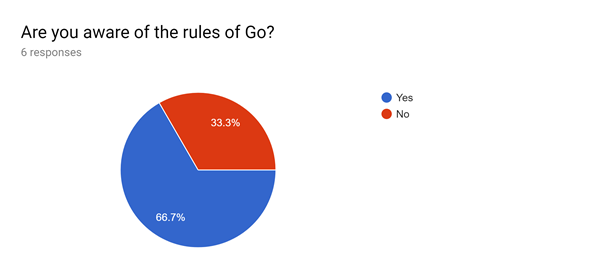
\includegraphics[width=\textwidth]{A1/1.png}
\end{subfigure}
\end{figure}

\begin{figure}[!ht]
\centering
\begin{subfigure}[b]{\textwidth}
\centering
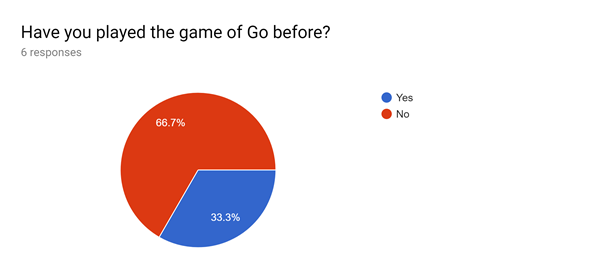
\includegraphics[width=\textwidth]{A1/2.png}
\end{subfigure}
\end{figure}


\begin{figure}[H]
\centering
\begin{subfigure}[b]{\textwidth}
\centering
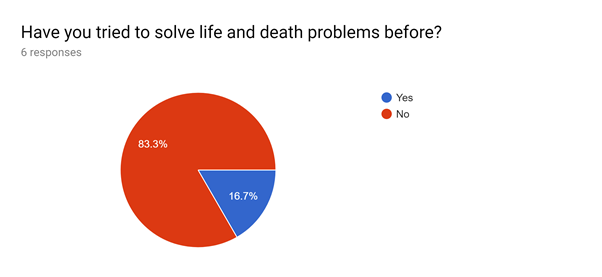
\includegraphics[width=\textwidth]{A1/3.png}
\end{subfigure}
\end{figure}

\section{Play Mode}

\begin{figure}[H]
\centering
\begin{subfigure}[b]{\textwidth}
\centering
\includegraphics[width=\textwidth]{A1/4.png}
\end{subfigure}
\end{figure}


\begin{figure}[H]
\centering
\begin{subfigure}[b]{\textwidth}
\centering
\includegraphics[width=\textwidth]{A1/5.png}
\end{subfigure}
\end{figure}


\begin{figure}[H]
\centering
\begin{subfigure}[b]{\textwidth}
\centering
\includegraphics[width=\textwidth]{A1/6.png}
\end{subfigure}
\end{figure}



\begin{figure}[H]
\centering
\begin{subfigure}[b]{\textwidth}
\centering
\includegraphics[width=\textwidth]{A1/7.png}
\end{subfigure}
\end{figure}


\begin{figure}[H]
\centering
\begin{subfigure}[b]{\textwidth}
\centering
\includegraphics[width=\textwidth]{A1/8.png}
\end{subfigure}
\end{figure}


\begin{figure}[H]
\centering
\begin{subfigure}[b]{\textwidth}
\centering
\includegraphics[width=\textwidth]{A1/9.png}
\end{subfigure}
\end{figure}

\section{Editor Mode}

\begin{figure}[H]
\centering
\begin{subfigure}[b]{\textwidth}
\centering
\includegraphics[width=\textwidth]{A1/10.png}
\end{subfigure}
\end{figure}


\begin{figure}[H]
\centering
\begin{subfigure}[b]{\textwidth}
\centering
\includegraphics[width=\textwidth]{A1/11.png}
\end{subfigure}
\end{figure}

\begin{figure}[H]
\centering
\begin{subfigure}[b]{\textwidth}
\centering
\includegraphics[width=\textwidth]{A1/12.png}
\end{subfigure}
\end{figure}

\begin{figure}[H]
\centering
\begin{subfigure}[b]{\textwidth}
\centering
\includegraphics[width=\textwidth]{A1/13.png}
\end{subfigure}
\end{figure}

\begin{figure}[H]
\centering
\begin{subfigure}[b]{\textwidth}
\centering
\includegraphics[width=\textwidth]{A1/14.png}
\end{subfigure}
\end{figure}



\begin{figure}[H]
\centering
\begin{subfigure}[b]{\textwidth}
\centering
\includegraphics[width=\textwidth]{A1/15.png}
\end{subfigure}
\end{figure}


\section{Solving Problems}

\begin{figure}[H]
\centering
\begin{subfigure}[b]{\textwidth}
\centering
\includegraphics[width=\textwidth]{A1-2/1.png}
\end{subfigure}
\end{figure}

\begin{figure}[H]
\centering
\begin{subfigure}[b]{\textwidth}
\centering
\includegraphics[width=\textwidth]{A1-2/2.png}
\end{subfigure}
\end{figure}



\begin{figure}[H]
\centering
\begin{subfigure}[b]{\textwidth}
\centering
\includegraphics[width=\textwidth]{A1-2/3.png}
\end{subfigure}
\end{figure}

\section{General}

\begin{figure}[H]
\centering
\begin{subfigure}[b]{\textwidth}
\centering
\includegraphics[width=\textwidth]{A1-2/4.png}
\end{subfigure}
\end{figure}

\begin{figure}[H]
\centering
\begin{subfigure}[b]{\textwidth}
\centering
\includegraphics[width=\textwidth]{A1-2/5.png}
\end{subfigure}
\end{figure}



\begin{figure}[H]
\centering
\begin{subfigure}[b]{\textwidth}
\centering
\includegraphics[width=\textwidth]{A1-2/6.png}
\end{subfigure}
\end{figure}

\chapter{User Guide}

\section{Menu}

\begin{figure}[H]
\centering
\begin{subfigure}[b]{\textwidth}
\centering
\includegraphics[width=\textwidth]{A3/1.png}
\caption{The menu screen}
\end{subfigure}
\end{figure}

Menu Screen contains three buttons. "Play Mode" enters play mode , to load and solve problems. "Editor Mode" enters editor ode , to create, edit and save problems. "Exit" quits out of the program.


\section{Play Mode}

\begin{figure}[H]
\centering
\begin{subfigure}[b]{\textwidth}
\centering
\includegraphics[width=\textwidth]{A3/2.png}
\caption{The menu screen}
\end{subfigure}
\end{figure}

Play Screen contains the Go board on the left and some controls on the right. The user can interact with the Go board by simply clicking on different points on the board to place a stone.
\subsection{Buttons}

Start: Tells the computer to start searching for the best move as the current colour.

Stop: Stops the computer in middle of the search, and makes the best move found so far in the search.

Undo: Reverts the board back to the previous state before the last move. (only goes back one move per click)

Redo: Reverts an undone move. (only goes forward one move per click)

Pass: Allows the user to pass – pass is disabled for attacking player unless no valid points of play due to Ko.

Reset: Goes back to the board state in which the board was loaded in.

Auto Play: Enable the computer to begin the search for a move immediately after you move.

Switch Turn: Changes the current turn to the opponent.


Limit Depth: If on, the computer only looks a set number of moves ahead before selecting a move. Otherwise it keeps searching until it finds a winning move or until there are no more moves to search.

Limit Breadth: If on, the computer only looks at the set number of valid moves at each depth. Otherwise looks at every valid move in each depth.


You can increase or decrease the breadth and depth using + or – buttons.
The number right of Limit Breadth is the breadth limit.
The number right of Limit Depth is the depth limit

Auto Play: Enable the computer to begin the search for a move immediately after you move.

Switch To Editor Mode: Enters editor mode. Wipes away the current board unless instead of switching back user goes to the menu and enter play mode.


Load : Allows you to load a problem.

Save : Allows you to save a problem mid way through.


\section{Editor Mode}

\begin{figure}[H]
\centering
\begin{subfigure}[b]{\textwidth}
\centering
\includegraphics[width=\textwidth]{A3/3.png}
\caption{The menu screen}
\end{subfigure}
\end{figure}

Editor Screen contains the Go board on the left and some controls on the right. The user can place stones on the board by simply clicking on the points of the board where they want stones.

\subsection{Buttons}

Place Black Stones : Switches the placing stone colour to be black.

Place White Stones : Switches the placing stone colour to be white.

Mark Valid Points : Switches the placing to a valid point marker. Used to set all valid points of the problem.

Remove Stones : Switches to deleting stones / valid points and replace them with an invalid point.


Black Keystone : Sets the keystone colour of the problem to black. This means black is the defending player.

White Keystone : Sets the keystone colour of the problem to white. This means white is the defending player.

Place KeyStone : Next stone to be placed is a keystone. Used to mark the objective of the problem. Capture keystone if you are the attacking player, proctect the keystone if you are the defending player.

Undo: Reverts the board back to the previous state before the last placement. (only goes back one placement per click)

Redo: Reverts an undone placement. (only goes forward one placement per click)

Flip V: Flips the board with line of horizontal symmetry.

Flip H: Flips the board with line of vertical  symmetry.

Rotate: Rotates the board in 90 degress.

Reset: Clears the entire board (cannot undo!)



Switch To Play Mode: Enters Play mode. Transfers the current board to play mode.

Load : Allows you to load a problem.

Save : Allows you to save a problem.

\section{Tutorial}

\subsection{Step by Step Tutorial}


\begin{enumerate}
\item Start the program.
\item A program window for Go-LD should appear.
\item This is the main menu, to begin choose “Play Mode”.
\item Here we can see a Go board on the left and some buttons on the right.
\item To load a problem to solve, press the load button.
\item From the Problems folder choose  “Tutorial.txt”.
\item The problem should be loaded on to the screen.
\item Few things to note:
\begin{itemize}

\item Stones appear on the board representing the problem inside the file.

\item Only the points outlined by circles are playable, these points are determined by the creator of the problem to discard irrelevant points on the board.

\item Either you or the computer can play first, “Start” tells the computer to play first or you can simply place a stone to begin.

\item Auto Play is enabled by default this means the computer automatically plays once you make a move.
\end{itemize}

\item You should play first by playing a stone at e1 - this move guarantees victory.

\item With Auto play on, the computer might have already a made a move at d1.

\item You might have noticed f1 is highlighted in red, this is because white cannot play there due to the self-capture rule.

\item At this point you can play anywhere and win , keep playing until you capture the black stones.

\item This is the basic idea behind the program to solve problems where the computer will try to play against you, you can also allow the computer to solve the problem and against you or itself.

\item Player v player,  player v computer or computer v computer are all possible within Go-LD using the buttons on the right of the screen.
\end{enumerate}


\end{appendices}


\bibliographystyle{abbrvnat}

\bibliography{Go_Project}



\end{document}
